\documentclass[11pt]{article}
\usepackage[margin=1in]{geometry}
\usepackage[T1]{fontenc}
\usepackage[utf8]{inputenc}
\usepackage{libertinus}
\usepackage{amsmath}
\usepackage{booktabs}
\usepackage{longtable}
\usepackage{tabularx}
\usepackage{array}
\usepackage{graphicx}
\usepackage{caption}
\usepackage{setspace}
\usepackage{xcolor}
\usepackage{xurl}
\usepackage{hyperref}
\usepackage[round]{natbib}
\usepackage{enumitem}
\usepackage{float}
\usepackage{fancyvrb}
\usepackage{fvextra}
\usepackage[most]{tcolorbox}
\usepackage{tikz}
\usetikzlibrary{arrows.meta,positioning,shapes.geometric,fit,calc,backgrounds,decorations.pathreplacing}

\definecolor{mfTreat}{HTML}{ED7354}
\definecolor{mfMedOne}{HTML}{457DEA}
\definecolor{mfMedTwo}{HTML}{C7953D}
\definecolor{mfOut}{HTML}{38A05E}
\definecolor{mfMissing}{HTML}{DB4A36}
\definecolor{mfPanelStroke}{HTML}{D6D6D1}
\definecolor{mfPanelFill}{HTML}{FFFFFF}
\definecolor{mfFigureBg}{HTML}{FCFBF9}
\definecolor{mfLabel}{HTML}{5E677D}
\definecolor{mfMuted}{HTML}{727D8F}

\setlength{\parskip}{0.55em}
\setlength{\parindent}{0pt}
\setlength{\emergencystretch}{1.5em}
\captionsetup{font=small,labelfont=bf}
\hypersetup{
  colorlinks=true,
  linkcolor=blue!50!black,
  urlcolor=blue!50!black,
  citecolor=blue!50!black
}

\newcommand{\repoURL}{\href{https://github.com/prashgarg/frontiergraph}{github.com/prashgarg/frontiergraph}}
\newcommand{\fignotes}[1]{\caption*{\textit{Notes.} #1}}
% WIP marker — renders in red bold; remove or replace with final content when done
\newcommand{\pendingnote}[1]{%
  \medskip\noindent\textcolor{red}{\textbf{[WIP: }\textit{#1}\textbf{]}}\medskip}
\newtcolorbox{promptbox}{
  enhanced,
  breakable,
  colback=gray!3,
  colframe=black!20,
  boxrule=0.4pt,
  arc=2pt,
  left=6pt,
  right=6pt,
  top=6pt,
  bottom=6pt
}
\newcommand{\promptfile}[1]{%
  \begin{promptbox}
  \VerbatimInput[fontsize=\tiny,breaklines=true,breakanywhere=true]{#1}
  \end{promptbox}
}
\newcolumntype{L}[1]{>{\raggedright\arraybackslash}p{#1}}
\newcolumntype{Y}{>{\raggedright\arraybackslash}X}

\title{\textbf{What Should Economics Ask Next?}\thanks{For helpful comments and discussions I thank Elliott Ash, Jasmin Baier, Thiemo Fetzer, Thomas Graeber, Paul H\"unermund, Ralf Martin, Chris Roth, Zekai Shen, and seminar participants at the CEPR--MPWZ Text-as-Data workshop. All remaining errors are my own.}}
\author{Prashant Garg\\[0.2em]\normalsize Imperial College London}
\date{12 April 2026\\[0.3em]\normalsize Draft for comments. Please do not cite without permission.}

\begin{document}
\maketitle
\onehalfspacing

\begin{abstract}
How should an economist choose which open question to work on next? I build a directed literature graph from 242{,}595 published economics-facing papers spanning 1976 to 2026, rank still-open candidate questions using only the graph available at each historical date, and test those rankings against later publication. A learned reranker built on that graph achieves a 17.0\% top-100 hit rate for mechanism-thickening questions and 10.7\% for direct-closure questions at a five-year horizon, versus 1.7\% for both under preferential attachment. The two families differ in what the screening recovers: mechanism-thickening yields denser shortlists, while direct-closure captures a larger share of all eventual realizations. These results establish that local literature structure contains useful upstream screening information---and that economics moves by deepening mechanisms around existing claims at roughly 3--12 times the rate at which it closes locally implied direct relations.
\end{abstract}

\textbf{Keywords:} research direction, economics of science, scientific discovery, question choice, literature graphs

\textbf{JEL codes:} O31, O33, C45, C81

\section{Introduction}

Choosing what to work on is one of the least formalized decisions in economics. We have disciplined tools for identification, estimation, and inference. We have much less guidance for the upstream choice of which question deserves scarce attention in the first place. Bloom et al.~\citeyearpar{bloom2020ideas} argue that ideas are getting harder to find, while Jones~\citeyearpar{jones2009burden} emphasizes the growing knowledge burden faced by new researchers. Those arguments point in the same direction: as the stock of published work grows, it becomes harder to see which question is worth pursuing next. Foster, Rzhetsky, and Evans~\citeyearpar{foster2015tradition} add a second concern. Scientists overwhelmingly choose conservative strategies even though riskier exploration disproportionately generates high-impact work. The problem is not only that question choice is hard. It is also tilted toward the familiar.

That problem becomes sharper when AI lowers the cost of downstream research tasks such as writing, background research, data analysis, and coding \citep{korinek2024generative}. Agrawal, McHale, and Oettl~\citeyearpar{agrawal2024ai} make the complementary point in a model of prioritized search: once ranking hypotheses becomes cheaper and better, the value of choosing what to test shifts further upstream. The question here is narrower than ``what should economics study?'' in the philosophical sense. It is whether the structure of past research can help rank candidate next questions in a disciplined way.

This paper builds a directed literature graph from 242{,}595 published economics-facing papers and tests whether that graph can predict which still-open questions later become part of the literature. At each historical date, I freeze the graph at \(t-1\), rank open candidate questions using only information available at that date, and check which ones appear in later published work. Comparing a popularity baseline, a transparent graph score, and a learned reranker, the answer is yes: a learned reranker achieves a 17.0\% top-100 hit rate for mechanism-thickening questions and 10.7\% for direct-closure questions at a five-year horizon, versus 1.7\% for both families under preferential attachment. The gains also differ in form. Mechanism-thickening yields denser shortlists (more later realizations per 100 suggestions), while direct-closure captures a larger share of all eventual realizations and ranks them earlier on average. The graph is therefore most useful as a tool for directing scarce reading time, not as a substitute for broad reading or field knowledge.

The paper studies two kinds of candidate question, which it calls \emph{direct-to-path} and \emph{path-to-direct}. In a direct-to-path case, the literature already contains a direct relation, but later work adds a clearer mechanism around it. In a path-to-direct case, the literature already contains nearby support for a relation, but the direct link itself is still missing and only appears later. These are different scientific moves. Direct-to-path asks where an accepted claim is still underexplained. Path-to-direct asks where nearby evidence already points toward a direct relation that the literature has not yet stated explicitly. An example: if the literature already links broadband access to business formation, later work adding a search-friction channel is a direct-to-path move. If the literature already connects trade liberalization to imported inputs and imported inputs to firm productivity, but has not yet stated a direct trade-to-productivity link, later work stating that link is a path-to-direct move.

The paper also documents the descriptive balance between these two motions. Economics more often adds mechanisms around existing claims than closes locally implied direct relations---at roughly 3--12 times the rate, depending on the horizon and era. That asymmetry is consistent with a scientific literature that deepens accepted lines rather than replaces them, and it bears on the interpretation of both shortlist families: the more abundant family is also the one for which the screening tool is most practically useful.

The roadmap is as follows. Section~\ref{sec:relatedlit} positions the paper in four related literatures. Section~\ref{sec:data} describes the corpus, extraction, and normalization pipeline. Section~\ref{sec:design} defines the two question objects, the transparent scoring rule, and the learned reranker. Section~\ref{sec:results} presents the paired shortlist comparison, the direct-to-path/path-to-direct asymmetry, and the reranker decomposition. Section~\ref{sec:discussion} interprets the findings and discusses implications. The appendix provides extraction details, full model comparisons, paired extensions showing the direct-to-path/path-to-direct trade-off across reading budgets, credibility audits, and supplementary usefulness checks.

\section{Related Literature}
\label{sec:relatedlit}

Four literatures bear on this paper, and the contribution is clearest against all four.

The first is the economics of ideas, discovery, and research direction. Bloom et al.~\citeyearpar{bloom2020ideas} document rising research effort alongside falling research productivity, while Jones~\citeyearpar{jones2009burden} studies how accumulating knowledge changes the organization of innovative activity.\footnote{The ``ideas are getting harder to find'' framing is itself debated. Fort et al.~\citeyearpar{fort2025growth} argue that what is declining is the translation of ideas into measured growth, not the rate of idea generation itself.} Those papers focus on the cost of reaching the frontier. However, a related literature asks whether incentives and norms steer researchers toward safe topics. Azoulay, Graff Zivin, and Manso~\citeyearpar{azoulay2011incentives} show that tolerating early failure produces more novel and high-impact work. Foster, Rzhetsky, and Evans~\citeyearpar{foster2015tradition} show that conservative strategies dominate in practice even though riskier exploration disproportionately generates breakthroughs.\footnote{Bhattacharya and Packalen~\citeyearpar{packalen2020stagnation} argue that citation-based incentives have further shifted scientists away from new ideas toward established topics, creating a self-reinforcing momentum that a screening tool could partially offset.} Although those papers study incentives at the system level, they motivate a narrower, operationally tractable question: given a large existing literature, can its local structure help screen candidate next questions in a way that is less path-dependent than cumulative advantage alone?

The second literature is science-of-science work using large-scale scientific data to study novelty, impact, and frontier formation. Fortunato et al.~\citeyearpar{fortunato2018science} and Wang and Barabasi~\citeyearpar{wang2021science} provide overviews of this field. Two specific findings are relevant here. Uzzi et al.~\citeyearpar{uzzi2013atypical} show that novelty often combines conventional structure with a small number of atypical combinations. Park, Leahey, and Funk~\citeyearpar{park2023disruptive} document a broad decline in disruptive science since the mid-twentieth century.\footnote{Petersen, Arroyave, and Pammolli~\citeyearpar{petersen2024disruption} argue that part of the measured decline reflects citation inflation rather than a real shift in innovativeness. For this paper, the relevant implication is narrower: whether or not measured disruption is declining, the literature's structure visibly thickens around existing claims over time, and that thickening is exactly what the path-development results in Section~\ref{sec:path-evolution} measure.} Although this literature is relevant in spirit, the empirical object here is different. I do not measure novelty from citations or reference-pair combinations. I define candidate next questions as missing links in a directed claim graph and evaluate them prospectively against later publication.

The third literature covers network growth, link prediction, and learning to rank. Price~\citeyearpar{price1976general} and Barabasi and Albert~\citeyearpar{barabasi1999emergence} show why already connected nodes tend to attract more links---a finding that here becomes the main null rather than a decorative comparison. The broader link-prediction literature \citep{liben2007link,martinez2016survey} and the learning-to-rank tradition \citep{liu2009learning} show that learned models can improve on fixed heuristics. More directly, recent work treats missing links in scientific knowledge graphs as candidate research directions. Krenn and Zeilinger~\citeyearpar{krenn2020predicting} and Gu and Krenn~\citeyearpar{gu2025impact4cast} propose knowledge-graph based discovery benchmarks; Sourati et al.~\citeyearpar{sourati2023accelerating} and Rzhetsky et al.~\citeyearpar{rzhetsky2015choosing} connect link prediction to scientific discovery. The present paper differs from all of these in three ways: it uses a directed economics claim graph, evaluates candidate questions in walk-forward vintages, and frames the problem as one of scarce reading time rather than generic link prediction. A nearby but distinct branch asks not which missing relation later appears, but which disconnected literatures or rising clusters are worth monitoring. Swanson's literature-based discovery program \citep{swanson1986upk} and emerging-topic systems \citep{blei2006dynamictopics,chen2006citespace,small2014emergingtopics} fall in this branch. The object here is more economist-facing: a ranked list of directed candidate questions evaluated against realized publication.

The fourth literature is AI-assisted scientific work. Recent systems help with hypothesis generation, literature synthesis, and manuscript support \citep{zhang2025scientificmethod,shao2025sciscigpt,korinek2024generative}.\footnote{Contemporary deployed examples include Refine (\url{https://www.refine.ink/}), the ICLR 2026 Reviewer Guide (\url{https://iclr.cc/Conferences/2026/ReviewerGuide}), Stanford Agentic Reviewer (\url{https://paperreview.ai/tech-overview}), and Project APE (\url{https://ape.socialcatalystlab.org/}). These are useful examples of the current tool landscape, but they are not treated as archival scholarly references in the bibliography.} Si, Yang, and Hashimoto~\citeyearpar{si2024llmideas} find that LLM-generated research ideas are rated more novel, though slightly less feasible, than expert-generated ones. Agrawal, McHale, and Oettl~\citeyearpar{agrawal2024ai} formalize AI-assisted discovery as prioritized search over a combinatorial hypothesis space. d'Aquin~\citeyearpar{daquin2025kgdiscovery} argues that knowledge graphs are becoming scaffolds for AI-based scientific discovery.\footnote{A related concern is that data-driven tools may narrow exploration rather than broaden it. Hoelzemann et al.~\citeyearpar{hoelzemann2024streetlight} show that when data highlights attractive but suboptimal paths, it can suppress breakthrough discovery. A screening tool has to be honest about that risk. The attention-frontier and heterogeneity results in the appendix speak to it directly.} The closest social-science comparisons in this space are Tong et al.~\citeyearpar{tong2024automating}, who extract causal relations from 43{,}312 psychology papers and use knowledge-graph link prediction to generate hypotheses, and Lee et al.~\citeyearpar{lee2024econcausal}, who construct a 10{,}490-triplet benchmark from economics and finance studies. The present paper differs in scale, in using prospective walk-forward evaluation rather than expert judgment, and in explicitly separating the benchmarkable historical object from the surfaced question---the human-readable candidate prompt built from the local graph neighborhood.

The present paper uses AI-extracted paper-level structure as an enabling layer and then asks an economics question: can that structure be turned into an inspectable, prospectively testable object for deciding what to read and work on next? Table~\ref{tab:positioning} summarizes how this paper differs from the closest comparable systems. The positioning is economics-first metascience with a graph-based empirical object, not a general-purpose AI assistant or a claim-extraction model.

\section{Data, Extraction, and Normalization}
\label{sec:data}

The sample covers 242{,}595 published economics-facing papers from 300 journals spanning 1976 to early 2026, at the directed concept-pair level. The pipeline extracts a paper-level claim graph from each title and abstract, matches repeated concept labels across papers into a shared node inventory, and then ranks missing directed links for prospective evaluation. Of those papers, 230{,}929 contain at least one extracted edge, yielding 1{,}443{,}407 raw extracted edges. After normalization and graph construction, the benchmark graph retains 230{,}479 papers and 1{,}271{,}014 normalized links. The frozen ontology---a fixed vocabulary of canonical concept labels used for cross-paper node matching and audit---contains 154{,}359 rows and is a separate object from the live benchmark graph. The next figures walk through the pipeline in order: one paper-level extraction, cross-paper matching into a shared graph, one live graph neighborhood, and the difference between the benchmark event and the richer question a reader inspects.

\subsection{Corpus}

The corpus covers the top 150 core economics journals and the top 150 adjacent journals, selected by field-weighted citation impact (FWCI). Work-level metadata, source metadata, and journal assignments come from OpenAlex.\footnote{OpenAlex enters the paper as the bibliographic and journal-metadata layer. The extraction, normalization, and ranking steps are built on top of that source rather than inherited from it.} The sample uses published journal papers rather than working papers, drafts, or preprints, because the goal is to study realized scientific structure in an economics-facing literature. That choice sacrifices some freshness in exchange for clearer source control, more stable metadata, and a graph that is easier to interpret as realized research rather than a mix of partially filtered text. The FWCI-based selection rule ties the retained sample to a published-literature core with credible economics or adjacent relevance. The corpus is not meant to exhaust the frontier. It defines a reproducible, interpretable literature against which missing links can be backtested. Appendix~\ref{app:benchmark-details} summarizes the corpus waterfall and retention numbers.

\begin{figure}[H]
  \caption{A paper excerpt and its local graph}
  \label{fig:extraction-flow}
  \centering
  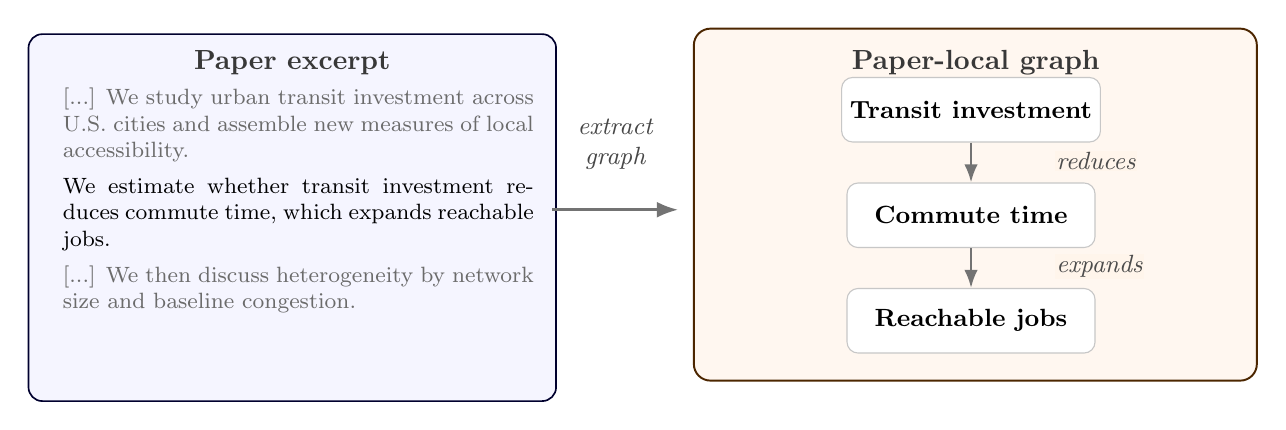
\begin{tikzpicture}[
    x=1cm, y=1cm,
    paperpanel/.style={draw=blue!18!black, rounded corners=5pt, fill=blue!4, line width=0.6pt},
    graphpanel/.style={draw=orange!30!black, rounded corners=6pt, fill=orange!6, line width=0.7pt},
    paneltitle/.style={font=\normalsize\bfseries, text=black!78},
    excerpt/.style={font=\footnotesize, align=justify, text width=5.98cm, inner sep=0pt},
    flownote/.style={font=\small\itshape, text=black!72},
    concept/.style={draw=black!22, rounded corners=4pt, fill=white, minimum width=3.15cm, minimum height=0.82cm, inner sep=3pt, font=\small\bfseries, align=center},
    relabel/.style={font=\small\itshape, text=black!70, fill=orange!10, fill opacity=0.38, text opacity=1, inner sep=0.45pt},
    flow/.style={-{Latex[length=2.7mm]}, draw=black!55, line width=1pt},
    edge/.style={-{Latex[length=2.3mm]}, draw=black!55, line width=0.9pt}
  ]
    \draw[paperpanel] (-0.25,-0.28) rectangle (6.45,4.38);
    \node[paneltitle] at (3.1,4.02) {Paper excerpt};
    \node[excerpt, anchor=north west] at (0.18,3.7) {%
      \textcolor{black!58}{[...] We study urban transit investment across U.S. cities and assemble new measures of local accessibility.}\par
      \vspace{0.42em}
      We estimate whether transit investment reduces commute time, which expands reachable jobs.\par
      \vspace{0.42em}
      \textcolor{black!58}{[...] We then discuss heterogeneity by network size and baseline congestion.}%
    };

    \draw[flow] (6.4,2.15) -- (8.0,2.15);
    \node[flownote, align=center] at (7.2,2.98) {extract\\graph};

    \draw[graphpanel] (8.2,-0.02) rectangle (15.35,4.45);
    \node[paneltitle] at (11.78,4.02) {Paper-local graph};

    \node[concept] (n1) at (11.72,3.42) {Transit investment};
    \node[concept] (n2) at (11.72,2.08) {Commute time};
    \node[concept] (n3) at (11.72,0.74) {Reachable jobs};

    \draw[edge] (n1) -- (n2);
    \draw[edge] (n2) -- (n3);
    \node[relabel, anchor=west] at (12.78,2.77) {reduces};
    \node[relabel, anchor=west] at (12.78,1.43) {expands};
  \end{tikzpicture}
  \fignotes{This figure isolates the extraction unit. One paper becomes one paper-local graph. The point is to show what is recovered before any cross-paper matching or normalization. The example is lightly cleaned from a live economics-facing transport-labor question, but the layout is stylized to make the extraction step legible.}
\end{figure}

\subsection{Paper-local graphs}

The extraction layer builds on Garg and Fetzer~\citeyearpar{gargfetzer2025causal}. Each title and abstract is converted into a paper-level graph in which nodes are extracted concepts and edges summarize the relations the paper itself states, studies, or reports (Figure~\ref{fig:extraction-flow}). The present paper extends that idea in three ways. First, the schema is broader than explicit causal claims, because the benchmark also needs undirected contextual support.\footnote{This is a deliberate departure from Garg and Fetzer~\citeyearpar{gargfetzer2025causal}. Their object is the rise of credible causal language and design in economics, so the stricter identified-causal layer is the natural headline object there. Here the downstream task is broader research allocation over candidate questions, so the main target is a wider causal-claim layer, while the stricter identified-causal layer is retained as a nested credibility-oriented benchmark.} Second, the schema separates the paper's \emph{causal presentation} from the \emph{evidence method} used to support a claim. Third, the graph stores contextual qualifiers in dedicated fields rather than forcing them into the node label. The goal is not just to recover whether a paper makes a claim. It is to recover enough local structure that the claim can later be used inside a reusable concept graph. Code, prompt files, and release materials are available in the public repository at \url{https://github.com/prashgarg/frontiergraph}.

The decision to work paper by paper first is deliberate. At extraction time, the task is not to solve global concept matching inside the language model. It is to recover each paper's own internal concept reuse faithfully and to prevent the model from inventing relations that are only implied by transitivity. Exact prompts, the full schema, and the design logic are reported in Appendix~\ref{app:extraction-protocol}. \textbf{The code and prompt files used in this paper will be released at \linebreak[2]\repoURL.}

\subsection{Node normalization}

Node normalization is central to the design because candidate generation, path counts, gap measures, and missingness all depend on node identity. Paper-local concept strings vary in wording, scope, and granularity. ``Inflation in Germany'', ``inflation'', and ``German inflation'' should not automatically remain three separate graph nodes if the downstream object is a reusable concept graph. But they should not be merged carelessly either.

For that reason the paper uses a fixed ontology and an auditable matching procedure rather than letting every paper-local label become its own global node or allowing unconstrained merging. The ontology combines JEL, an economics-filtered Wikidata pull, OpenAlex topics, OpenAlex keywords, and an economics-filtered Wikipedia crawl. The frozen baseline contains 154{,}359 rows. Matching then proceeds in stages. Exact lexical cases are resolved deterministically first. Harder cases use embedding retrieval, but the system keeps multiple candidates and reviewed overlays rather than forcing one irreversible merge.\footnote{The embedding step is used as a retrieval and ranking device after exact lexical passes, not as an unconstrained merge rule. That ordering keeps obvious cases deterministic and makes softer matches auditable.} The practical aim is simple: merge obvious duplicates, avoid false precision, and keep uncertain cases visible for later audit rather than hiding them inside one aggressive normalization pass. Appendix~\ref{app:node-normalization} gives the full algorithm and the retention counts. Table~\ref{tab:notation} fixes the key notation used throughout the paper.

\begin{figure}[H]
  \caption{Cross-paper matching reveals a shared candidate neighborhood}
  \label{fig:shared-candidate-formation}
  \centering
  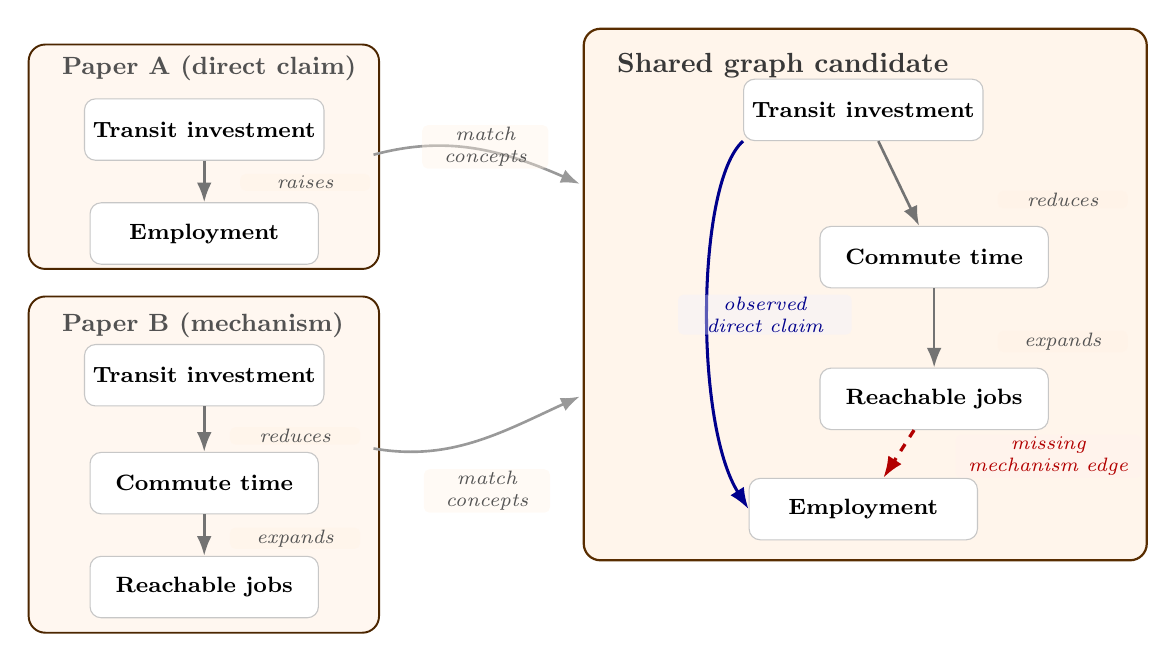
\begin{tikzpicture}[
    x=1cm, y=1cm,
    paperpanel/.style={draw=orange!30!black, rounded corners=6pt, fill=orange!6, line width=0.7pt},
    graphpanel/.style={draw=orange!35!black, rounded corners=6pt, fill=orange!8, line width=0.8pt},
    panelhead/.style={font=\normalsize\bfseries, text=black!78},
    paperhead/.style={font=\small\bfseries, text=black!68},
    concept/.style={draw=black!22, rounded corners=4pt, fill=white, minimum width=2.9cm, minimum height=0.78cm, inner sep=3pt, font=\footnotesize\bfseries, align=center},
    causal/.style={-{Latex[length=2.5mm]}, draw=black!55, line width=0.95pt},
    directclaim/.style={-{Latex[length=2.7mm]}, draw=blue!55!black, line width=1.1pt},
    missedge/.style={-{Latex[length=2.7mm]}, draw=red!70!black, line width=1.2pt, dashed},
    matcher/.style={-{Latex[length=2.4mm]}, draw=black!40, line width=0.95pt},
    edgelabel/.style={font=\scriptsize\itshape, text=black!67, fill=orange!10, fill opacity=0.38, text opacity=1, rounded corners=2pt, inner sep=0.75pt, align=center, text width=1.6cm},
    bluelabel/.style={font=\scriptsize\itshape, text=blue!55!black, fill=blue!6, fill opacity=0.38, text opacity=1, rounded corners=2pt, inner sep=0.8pt, align=center, text width=2.15cm},
    redlabel/.style={font=\scriptsize\itshape, text=red!70!black, fill=red!6, fill opacity=0.38, text opacity=1, rounded corners=2pt, inner sep=0.8pt, align=center, text width=2.3cm}
  ]
    \draw[paperpanel] (0,3.9) rectangle (4.45,6.75);
    \node[paperhead, anchor=west] at (0.3,6.45) {Paper A (direct claim)};
    \node[concept] (a1) at (2.23,5.67) {Transit investment};
    \node[concept] (a2) at (2.23,4.35) {Employment};
    \draw[causal] (a1) -- (a2);
    \node[edgelabel, anchor=west] at (2.68,5.0) {raises};

    \draw[paperpanel] (0,-0.72) rectangle (4.45,3.55);
    \node[paperhead, anchor=west] at (0.3,3.18) {Paper B (mechanism)};
    \node[concept] (b1) at (2.23,2.55) {Transit investment};
    \node[concept] (b2) at (2.23,1.18) {Commute time};
    \node[concept] (b3) at (2.23,-0.14) {Reachable jobs};
    \draw[causal] (b1) -- (b2);
    \draw[causal] (b2) -- (b3);
    \node[edgelabel, anchor=west] at (2.55,1.78) {reduces};
    \node[edgelabel, anchor=west] at (2.55,0.48) {expands};

    \draw[matcher] (4.38,5.35) .. controls (5.3,5.6) and (6.0,5.42) .. (7.0,4.98);
    \draw[matcher] (4.38,1.62) .. controls (5.35,1.45) and (6.0,1.82) .. (7.0,2.28);
    \node[edgelabel, text width=1.55cm] at (5.8,5.45) {match concepts};
    \node[edgelabel, text width=1.55cm] at (5.82,1.08) {match concepts};

    \draw[graphpanel] (7.05,0.2) rectangle (14.2,6.95);
    \node[panelhead, anchor=west] at (7.35,6.48) {Shared graph candidate};

    \node[concept] (g1) at (10.6,5.92) {Transit investment};
    \node[concept] (g2) at (11.5,4.05) {Commute time};
    \node[concept] (g3) at (11.5,2.25) {Reachable jobs};
    \node[concept] (g4) at (10.6,0.85) {Employment};

    \draw[causal] (g1) -- (g2);
    \draw[causal] (g2) -- (g3);
    \draw[directclaim] (g1.south west) .. controls (8.48,5.0) and (8.45,1.95) .. (g4.west);
    \draw[missedge] (g3) -- (g4);

    \node[edgelabel, anchor=west] at (12.3,4.78) {reduces};
    \node[edgelabel, anchor=west] at (12.3,2.98) {expands};
    \node[bluelabel] at (9.35,3.32) {observed\\direct claim};
    \node[redlabel] at (12.95,1.52) {missing\\mechanism edge};
  \end{tikzpicture}
  \fignotes{This figure isolates the cross-paper step. The two left panels are separate paper-local graphs. Only after repeated labels are matched into shared concepts does the right panel exist. The example is a direct-to-path case: one paper contributes a direct claim, another contributes a mechanism fragment, and the shared graph reveals a missing mechanism edge that can be benchmarked prospectively.}
\end{figure}

\begin{table}[t]
  \caption{Core notation used in the paper}
  \label{tab:notation}
  \centering
  \begin{tabular}{L{0.18\linewidth}L{0.74\linewidth}}
    \toprule
    Symbol & Definition \\
    \midrule
    \(G_{t-1}=(V,E_{t-1})\) & Claim graph assembled from papers observed through year \(t-1\). It contains directed causal links and undirected contextual support inside one concept-level graph object. \\
    \(u,v,w\) & Normalized concept nodes in the ontology-backed graph. \\
    \(u \rightarrow v\) & Directed causal link or directed causal candidate. \\
    \(\{u,v\}\) & Undirected noncausal pair. \\
    \(h\) & Evaluation horizon in years. \\
    \(K\) & Shortlist size in the fixed-budget retrieval problem. \\
    \bottomrule
  \end{tabular}
  \fignotes{This table collects the symbols used repeatedly in the benchmark and scoring sections. The dated graph \(G_{t-1}\) is always the graph observed through year \(t-1\), so every score, feature, and candidate is constructed without seeing papers from year \(t\) or later. \(h\) is the forecast window in years, and \(K\) is the number of candidate links or surfaced questions a reader is willing to inspect.}
\end{table}

\begin{figure}[t]
  \caption{A local neighborhood from the live graph}
  \label{fig:real-neighborhood}
  \centering
  \includegraphics[width=0.92\linewidth]{real_neighborhood.png}
  \fignotes{The previous figures are conceptual examples. This figure is a real neighborhood from the live graph, built around the candidate \emph{Trade Liberalization \(\rightarrow\) R\&D}. Blue arrows are directed causal edges; gray lines are undirected contextual support. The figure is not a result in itself. Its job is to show that the benchmark ultimately operates on graph neighborhoods of this kind rather than on hand-drawn concept diagrams.}
\end{figure}

\section{Question Objects and Evaluation}
\label{sec:design}

A natural first instinct is to ask a large language model directly: list the concept pairs likely to be studied next, or judge whether a given pair will be connected. The difficulty is one of evaluation rather than prediction. A general-purpose model has been trained on much of the period one would hope to predict, so any accuracy figure is confounded by leakage from the test window into the training corpus \citep{kapoor2023leakage,carlini2023memorization}. It has no calibrated base rate at which pairs become linked, so shortlists cannot be compared against a top-\(K\) realization count. And it cannot be re-run at strict pre-training cutoffs, which rules out walk-forward evaluation. Semantic-similarity baselines over concept embeddings inherit the same problems. What follows in this section is designed around those constraints: a dated support graph, a transparent structural score, and a learned reranker evaluated walk-forward against realized future links.

The historical backtest requires separating two objects: the dated graph event that can be tested prospectively, and the reader-facing question built from the same neighborhood. Figure~\ref{fig:real-neighborhood} shows one real neighborhood of the underlying concept graph. The remainder of this section makes the distinction precise.

\subsection{Two question objects}
\label{sec:missing-links}

The graph supports two historical families of candidate question. In a \emph{direct-to-path} case, the literature already contains a direct relation at date \(t-1\), but the surrounding mechanism is still thin. Later work adds a mediating path around that relation. In a \emph{path-to-direct} case, the literature already contains a local path at date \(t-1\), but the direct relation itself is still missing. Later work states that direct relation explicitly.

The distinction matters because the two families ask different things of a literature. Direct-to-path asks where an accepted relation is still underexplained. Path-to-direct asks where nearby evidence already points to a direct claim the literature has not yet stated. Direct-to-path is the more immediately readable family for most economists, since much empirical work moves from reduced-form relations to channels, heterogeneity, and scope conditions. But path-to-direct matters too: some later papers close a missing direct relation rather than only elaborate an accepted claim.

The headline benchmark is directed. At cutoff \(t\), the candidate universe is the set of directed causal links that are still missing from the graph observed through year \(t-1\). Undirected contextual support remains important: it scores and interprets the directed candidates without itself being ranked.

For the directed causal task, the candidate universe at cutoff \(t\) is
\[
\mathcal{C}^{D}_{t}=\{(u,v)\in V\times V: u\neq v,\ (u\rightarrow v)\notin E^{D}_{t-1}\},
\]
where \(E^{D}_{t-1}\) denotes the directed causal subgraph observed through year \(t-1\). A future realization occurs when \(u \rightarrow v\) first appears during \([t,t+h]\). At each cutoff, take the active concepts, form all ordered source-target pairs, and drop any pair whose directed causal edge is already in the graph. What remains is the set of still-missing direct claims the paper can rank at date \(t\). A candidate counts as realized only when that direct claim first appears within the horizon window, not when the concepts merely keep co-appearing.

The historical event and the surfaced question are not the same. The historical event is whether the relevant direct edge or path appears later in the graph. The surfaced question is the human-readable prompt built around the local neighborhood. That separation matters because economists do not browse bare graph events. They browse questions that could plausibly become papers (Figure~\ref{fig:candidate-schematic}).

The surfaced question stays centered on the endpoints---or on the endpoints plus one mediator---because the benchmark requires one dated event and the reader needs one inspectable question. A fuller local neighborhood may contain several paths and overlapping readings, but those richer motifs enter as supporting evidence rather than as the event itself.

The main backtest also holds the active concept set fixed at the cutoff. A distinct extension is \emph{node activation}: dormant ontology concepts, weakly grounded phrases, or genuinely new concepts entering the active graph later. That object matters, but it requires a different dated event than missing-link appearance and is therefore better treated as a separate frontier problem.

\begin{figure}[H]
  \caption{The benchmark anchor is narrower than the surfaced question}
  \label{fig:candidate-schematic}
  \centering
  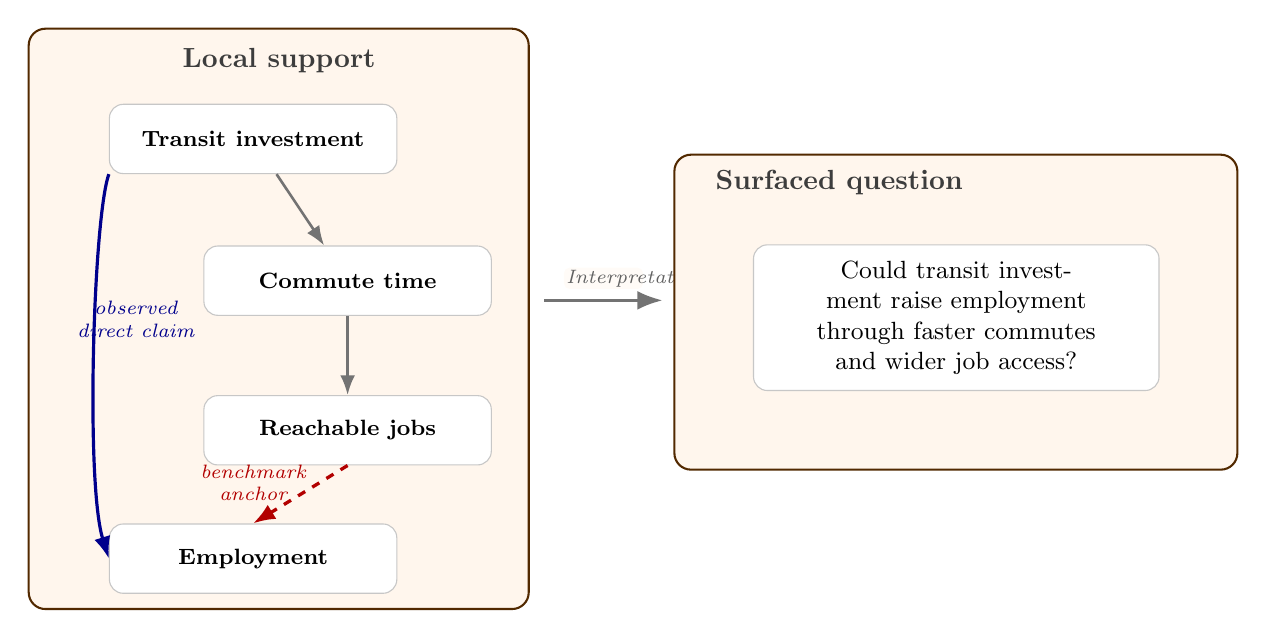
\begin{tikzpicture}[
    x=1cm,y=1cm,
    panel/.style={draw=orange!32!black, rounded corners=6pt, fill=orange!7, line width=0.75pt},
    panelhead/.style={font=\normalsize\bfseries, text=black!76},
    concept/.style={draw=black!22, rounded corners=5pt, fill=white, minimum width=3.65cm, minimum height=0.88cm, inner sep=3pt, font=\footnotesize\bfseries, align=center},
    qbox/.style={draw=black!22, rounded corners=5pt, fill=white, minimum width=5.15cm, minimum height=1.85cm, inner sep=5pt, font=\small, align=center, text width=4.55cm},
    causal/.style={-{Latex[length=2.5mm]}, draw=black!55, line width=0.95pt},
    directclaim/.style={-{Latex[length=2.8mm]}, draw=blue!55!black, line width=1.15pt},
    missedge/.style={-{Latex[length=2.8mm]}, draw=red!70!black, line width=1.2pt, dashed},
    compress/.style={-{Latex[length=3.2mm]}, draw=black!55, line width=1.05pt},
    blabel/.style={font=\scriptsize\itshape, text=blue!55!black, align=center},
    rlabel/.style={font=\scriptsize\itshape, text=red!70!black, align=center},
    flowlabel/.style={font=\scriptsize\itshape, text=black!62, fill=orange!8, fill opacity=0.38, text opacity=1, rounded corners=2pt, inner sep=0.8pt, align=center, text width=0.95cm}
  ]
    \draw[panel] (0,-0.82) rectangle (6.35,6.55);
    \node[panelhead] at (3.18,6.15) {Local support};

    \node[concept] (l1) at (2.85,5.15) {Transit investment};
    \node[concept] (l2) at (4.05,3.35) {Commute time};
    \node[concept] (l3) at (4.05,1.45) {Reachable jobs};
    \node[concept] (l4) at (2.85,-0.18) {Employment};

    \draw[causal] (l1) -- (l2);
    \draw[causal] (l2) -- (l3);
    \draw[directclaim] (l1.south west) .. controls (0.82,4.15) and (0.72,0.78) .. (l4.west);
    \draw[missedge] (l3.south) -- (l4.north);

    \node[blabel] at (1.36,2.86) {observed\\direct claim};
    \node[rlabel] at (2.85,0.78) {benchmark\\anchor};

    \draw[compress] (6.55,3.1) -- (8.05,3.1);
    \node[flowlabel] at (7.3,3.38) {Interpretation};

    \draw[panel] (8.2,0.95) rectangle (15.35,4.95);
    \node[panelhead, anchor=west] at (8.6,4.6) {Surfaced question};
    \node[qbox] at (11.78,2.88) {Could transit investment raise employment\\
    through faster commutes\\
    and wider job access?};
  \end{tikzpicture}
  \fignotes{The dashed edge inside the left panel is the benchmark anchor that can be backtested. The reader-facing question is richer: it keeps that same anchor but presents the surrounding support graph as a readable question. The surfaced question is therefore a compression of the neighborhood evidence, not the benchmark event itself.}
\end{figure}

\subsection{Gap and boundary questions}

Two kinds of surfaced questions matter in practice. Gap questions already have rich nearby support but remain directly underworked. Boundary questions connect areas that still have little direct traffic between them. The paper's score is designed to separate these cases rather than collapse them into one novelty index. Gap questions are often easier to defend as plausible next questions; boundary questions are often more adventurous and potentially more fragile.

\begin{figure}[p]
  \caption{Gap and boundary questions are different local graph patterns}
  \label{fig:gap-boundary}
  \centering
  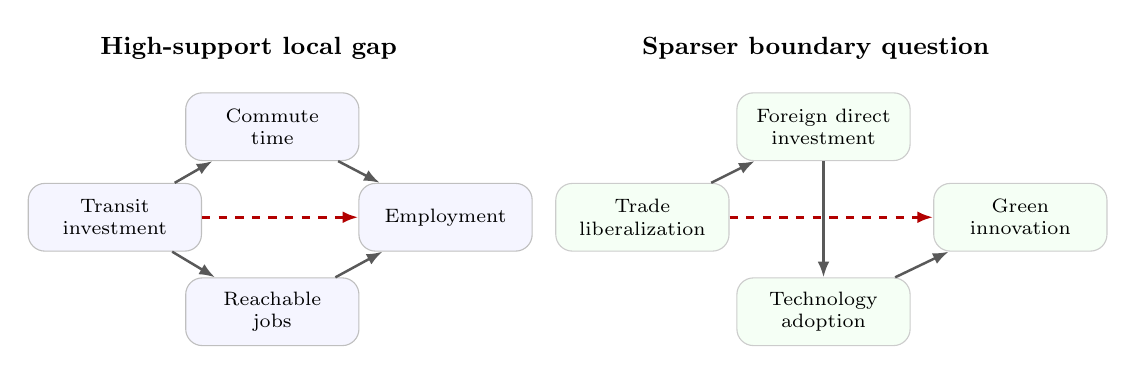
\begin{tikzpicture}[
    x=1cm,y=1cm,
    node/.style={draw=black!25, rounded corners=6pt, fill=blue!4, minimum width=2.2cm, minimum height=0.86cm, inner sep=2pt, align=center, font=\scriptsize},
    lightnode/.style={draw=black!20, rounded corners=6pt, fill=green!4, minimum width=2.2cm, minimum height=0.86cm, inner sep=2pt, align=center, font=\scriptsize},
    edge/.style={-{Latex[length=2mm]}, draw=black!65, line width=0.9pt},
    miss/.style={-{Latex[length=2mm]}, draw=red!70!black, dashed, line width=1.1pt}
  ]
    \node[font=\small\bfseries] at (2.5,4.35) {High-support local gap};
    \node[node] (d1) at (0.8,2.2) {Transit\\investment};
    \node[node] (i1) at (2.8,3.35) {Commute\\time};
    \node[node] (f1) at (2.8,1.0) {Reachable\\jobs};
    \node[node] (c1) at (5.0,2.2) {Employment};
    \draw[edge] (d1) -- (i1);
    \draw[edge] (i1) -- (c1);
    \draw[edge] (d1) -- (f1);
    \draw[edge] (f1) -- (c1);
    \draw[miss] (d1) -- (c1);

    \node[font=\small\bfseries] at (9.7,4.35) {Sparser boundary question};
    \node[lightnode] (t2) at (7.5,2.2) {Trade\\liberalization};
    \node[lightnode] (g2) at (9.8,3.35) {Foreign direct\\investment};
    \node[lightnode] (f2) at (9.8,1.0) {Technology\\adoption};
    \node[lightnode] (e2) at (12.3,2.2) {Green\\innovation};
    \draw[edge] (t2) -- (g2);
    \draw[edge] (g2) -- (f2);
    \draw[edge] (f2) -- (e2);
    \draw[miss] (t2) -- (e2);
  \end{tikzpicture}
  \fignotes{This figure exists to separate two screening cases that would otherwise look similar in prose. The left panel shows a gap-like candidate: nearby support is already dense, but the direct relation remains missing. The right panel shows a more boundary-like candidate: the two end concepts are connected only by a thinner mechanism chain. The node labels are hand-curated economics-facing examples used only to make the local graph pattern readable. The diagrams are conceptual rather than exhaustive.}
\end{figure}

In the language of the graph, gap questions have high local support and low direct completion. Boundary questions have weaker local closure but connect parts of the graph that are still far apart. The gap-boundary split matters for interpreting the screening results: the reranker surfaces a different gap-boundary mix than the popularity benchmark (Section~\ref{sec:results}).

\subsection{Transparent scoring rule}

The ranking rule combines four ingredients: path support, underexploration gap, motif
support, and hub penalty. Using the same transit-investment example that runs through the
earlier method figures, path support asks whether the two endpoint concepts are already
connected by short routes through nearby mediators. The gap term asks whether those routes
exist even though the direct relation itself is still absent or thin. Motif support asks
whether the same endpoint pair keeps reappearing inside nearby structural patterns rather
than in only one fragile corner of the graph. The hub penalty moves in the opposite
direction: it reduces scores that are high only because both endpoints are extremely
generic, heavily connected concepts.

\begin{figure}[t]
  \caption{The transparent score rewards supported but still undercompleted pairs}
  \label{fig:score-components}
  \centering
  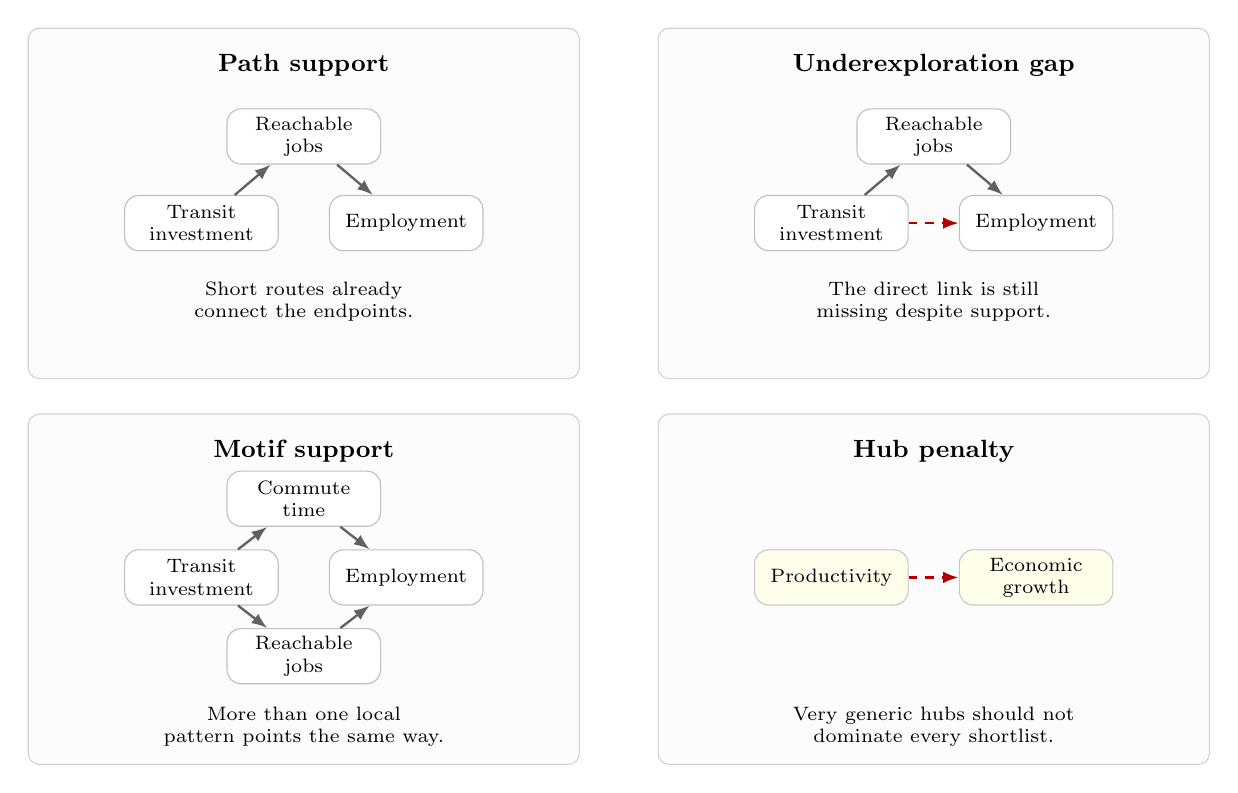
\begin{tikzpicture}[
    x=1cm,y=1cm,
    panel/.style={draw=black!18, rounded corners=4pt, fill=gray!2, minimum width=7.0cm, minimum height=4.45cm},
    node/.style={draw=black!25, rounded corners=5pt, fill=white, minimum width=1.95cm, minimum height=0.7cm, inner sep=2pt, font=\scriptsize, align=center},
    hub/.style={draw=black!22, rounded corners=5pt, fill=yellow!8, minimum width=1.95cm, minimum height=0.7cm, inner sep=2pt, font=\scriptsize, align=center},
    edge/.style={-{Latex[length=2mm]}, draw=black!62, line width=0.85pt},
    miss/.style={-{Latex[length=2mm]}, draw=red!70!black, dashed, line width=1.0pt},
    lab/.style={font=\small\bfseries}
  ]
    \node[panel] at (4.1,5.2) {};
    \node[panel] at (12.1,5.2) {};
    \node[panel] at (4.1,0.3) {};
    \node[panel] at (12.1,0.3) {};
    \node[lab] at (4.1,6.95) {Path support};
    \node[lab] at (12.1,6.95) {Underexploration gap};
    \node[lab] at (4.1,2.05) {Motif support};
    \node[lab] at (12.1,2.05) {Hub penalty};

    \node[node] (k1) at (2.8,4.95) {Transit\\investment};
    \node[node] (k2) at (4.1,6.05) {Reachable\\jobs};
    \node[node] (k3) at (5.4,4.95) {Employment};
    \draw[edge] (k1) -- (k2);
    \draw[edge] (k2) -- (k3);
    \node[font=\scriptsize, align=center] at (4.1,3.95) {Short routes already\\connect the endpoints.};

    \node[node] (l1) at (10.8,4.95) {Transit\\investment};
    \node[node] (l2) at (12.1,6.05) {Reachable\\jobs};
    \node[node] (l3) at (13.4,4.95) {Employment};
    \draw[edge] (l1) -- (l2);
    \draw[edge] (l2) -- (l3);
    \draw[miss] (l1) -- (l3);
    \node[font=\scriptsize, align=center] at (12.1,3.95) {The direct link is still\\missing despite support.};

    \node[node] (m1) at (2.8,0.45) {Transit\\investment};
    \node[node] (m2) at (4.1,1.45) {Commute\\time};
    \node[node] (m3) at (4.1,-0.55) {Reachable\\jobs};
    \node[node] (m4) at (5.4,0.45) {Employment};
    \draw[edge] (m1) -- (m2);
    \draw[edge] (m2) -- (m4);
    \draw[edge] (m1) -- (m3);
    \draw[edge] (m3) -- (m4);
    \node[font=\scriptsize, align=center] at (4.1,-1.45) {More than one local\\pattern points the same way.};

    \node[hub] (n1) at (10.8,0.45) {Productivity};
    \node[hub] (n2) at (13.4,0.45) {Economic\\growth};
    \draw[miss] (n1) -- (n2);
    \node[font=\scriptsize, align=center] at (12.1,-1.45) {Very generic hubs should not\\dominate every shortlist.};
  \end{tikzpicture}
  \fignotes{This figure makes the transparent score legible without the formula. The first three panels continue the same transit-investment worked example used in the earlier method figures. Path support asks whether short routes already connect the endpoints. The underexploration gap asks whether the direct relation is still missing despite that support. Motif support asks whether more than one nearby pattern points toward the same endpoint pair. The final panel intentionally switches to generic hubs to show the opposite force: the score should not rank a candidate highly only because both concepts are broad and heavily connected.}
\end{figure}

Formally, the score for a candidate pair \((u,v)\) is a weighted sum of four components:
\[
s(u,v)=\alpha \tilde P(u,v)+\beta G(u,v)+\gamma \tilde M(u,v)-\delta \tilde H(u,v),
\]
where \(\tilde P(u,v)\) is normalized path support, \(G(u,v)\) is the underexploration gap,
\(\tilde M(u,v)\) is normalized motif support, and \(\tilde H(u,v)\) is the normalized hub
penalty. The main specification uses \(\alpha=0.5\), \(\beta=0.2\), \(\gamma=0.3\), and
\(\delta=0.2\). Those
weights are fixed by design rather than tuned to maximize forecasting
performance. A pair scores highly when several nearby routes keep pointing toward it, the
direct relation still looks oddly absent relative to that support, and the pair is not
simply another generic high-degree combination. Figures~\ref{fig:gap-boundary}
and~\ref{fig:score-components} show directly what the rule rewards: multiple short paths,
repeated local support, and a direct link that still looks underfilled relative to its
neighborhood.
The notation is easier to read if each term is treated as answering one question. Is there
already short local support connecting the endpoints? That is \(\tilde P\). Does the direct
claim still look missing relative to that support? That is \(G\). Is the signal repeated in
more than one nearby motif rather than hanging on one fragile path? That is \(\tilde M\). Are
the endpoints simply very generic hubs that would connect to almost anything? That is
\(\tilde H\), which is subtracted rather than added. So the score is not an opaque index. It is
a transparent compromise between support, missingness, repeated local confirmation, and a
penalty for generic popularity.

That transparency choice matters for interpretation. The graph already stores stability,
causal-presentation, evidence-type, and edge-role metadata, but the main score does not yet
fully weight those signals. That choice is deliberate. The score is meant to be inspectable question by question rather
than optimized as a forecasting black box, and richer credibility weighting is better
understood as the next extension than as a hidden tuning layer.

\subsection{Learned reranker}
\label{sec:reranker-design}

The transparent score is fixed-weight and inspectable. Its weights are chosen by design rather than tuned to historical outcomes, which keeps the score readable question by question. The cost is that fixed weights may miss combinations of graph features that matter for screening. The learned reranker asks a narrower question: if the candidate set and time discipline stay fixed, does a model that learns how to weight the same graph information improve the shortlist? The reranker uses the same missing-link candidates, only information available at the historical cutoff, and no text, author, or institutional features.

\paragraph{Feature families.}
The reranker uses five nested feature families. The base is the transparent graph score itself. Two further families add local graph structure---path support, motif counts, mediator counts, co-occurrence signals, endpoint degree products, and a same-field indicator---and timing signals: support age, recency of the most recent supporting edge, and recent-window degree and incident counts for each endpoint. The final two families cover evidence composition (mean edge stability, evidence-type diversity, venue diversity, source diversity, and mean field-weighted citation impact at each endpoint) and boundary and gap indicators (whether the endpoints sit in different field groups with no co-occurrence, whether the pair looks gap-like, and the local closure density around the pair). The richest specification uses 34 graph-derived features; Table~\ref{tab:feature-families} in Appendix~\ref{app:reranker-design} lists the full inventory. The ordering is cumulative so each nested specification's marginal contribution can be isolated.

\paragraph{Training design.}
Training follows the same walk-forward discipline as the main benchmark. At each evaluation cutoff \(t\), the model is trained only on earlier cutoff-year cells and is evaluated at \(t\). Features are computed from the historical corpus through year \(t-1\). The positive label is whether the candidate edge first appears within the evaluation horizon. I test two model families: logistic regression with class-balanced weights, and a pairwise ranking model trained on positive-versus-negative feature differences. Both use \(L_2\) regularization. Because the feature families are nested, the paper can ask a simple question at each step: does adding more graph information improve screening beyond topology alone? Appendix~\ref{app:reranker-design} gives the full training design, regularization grid, best configurations by horizon, and grouped feature decompositions.

\paragraph{Scope.}
The reranker stays inside the graph-screening framing: every feature comes from the literature graph (no text, no author identity, no external data), the candidate set is the same set of missing links, and the temporal discipline is the same walk-forward design.\footnote{The difference is only in how the graph features are combined: by fixed design judgment in the transparent score, or by weights learned from earlier cutoffs in the reranker. A separate design question is how far out in the support graph to look when generating candidates. The main benchmark uses \texttt{max\_path\_len = 3}, allowing paths of length two (one mediator) and three (two mediators). Appendix~\ref{app:path-length-axis} documents the sensitivity of the results to that choice, comparing path lengths 2 and 3 on the same tuned pipeline. Appendix~\ref{app:path-length-illustrations} makes that comparison concrete with four curated endpoint pairs (one per cluster), and Appendix~\ref{app:path-length-illustrations-sweep} extends the illustration to full per-source top-20 target sweeps for eight anchor concepts. Appendix~\ref{app:reranker-design} includes a Shapley-value decomposition showing which features drive the combined model's predictions.}

\subsection{Walk-forward evaluation}

The prospective design freezes the graph at year \(t-1\), ranks candidates using only information available at that date, and checks whether those links first appear over the evaluation horizon.\footnote{The model at year \(t-1\) cannot use information from papers appearing in \(t\) or later---that is the sense in which the design avoids leakage.} This keeps the benchmark close to the ex ante decision problem rather than retrospective fit. The question is not ``how well does the score fit the historical graph?'' but ``how well would this score have surfaced links that later became realized work?'' Retrospective fit can reward mechanical regularities that carry no information about research allocation; the walk-forward design cannot.

For each cutoff year, the graph is built from the historical stock only. Realizations are then defined from future papers over the chosen horizon. The benchmark is rolling rather than one-shot, so each horizon is evaluated across multiple cutoff dates. A cutoff is eligible for horizon \(h\) only if \(t+h\leq 2026\); the appendix horizon extension applies the same rule on a five-year cutoff grid when it extends the transparent benchmark to \(h=20\). The headline benchmark focuses on directed causal candidates. The fuller atlas also evaluates directed and undirected objects separately and pools them by weighted aggregation rather than constructing one mixed ranking universe. Figure~\ref{fig:evaluation-design} makes the temporal discipline visual.

\begin{figure}[p]
  \caption{Walk-forward evaluation keeps scoring vintage-correct}
  \label{fig:evaluation-design}
  \centering
  \makebox[\linewidth][c]{%
  \resizebox{1.04\linewidth}{!}{%
  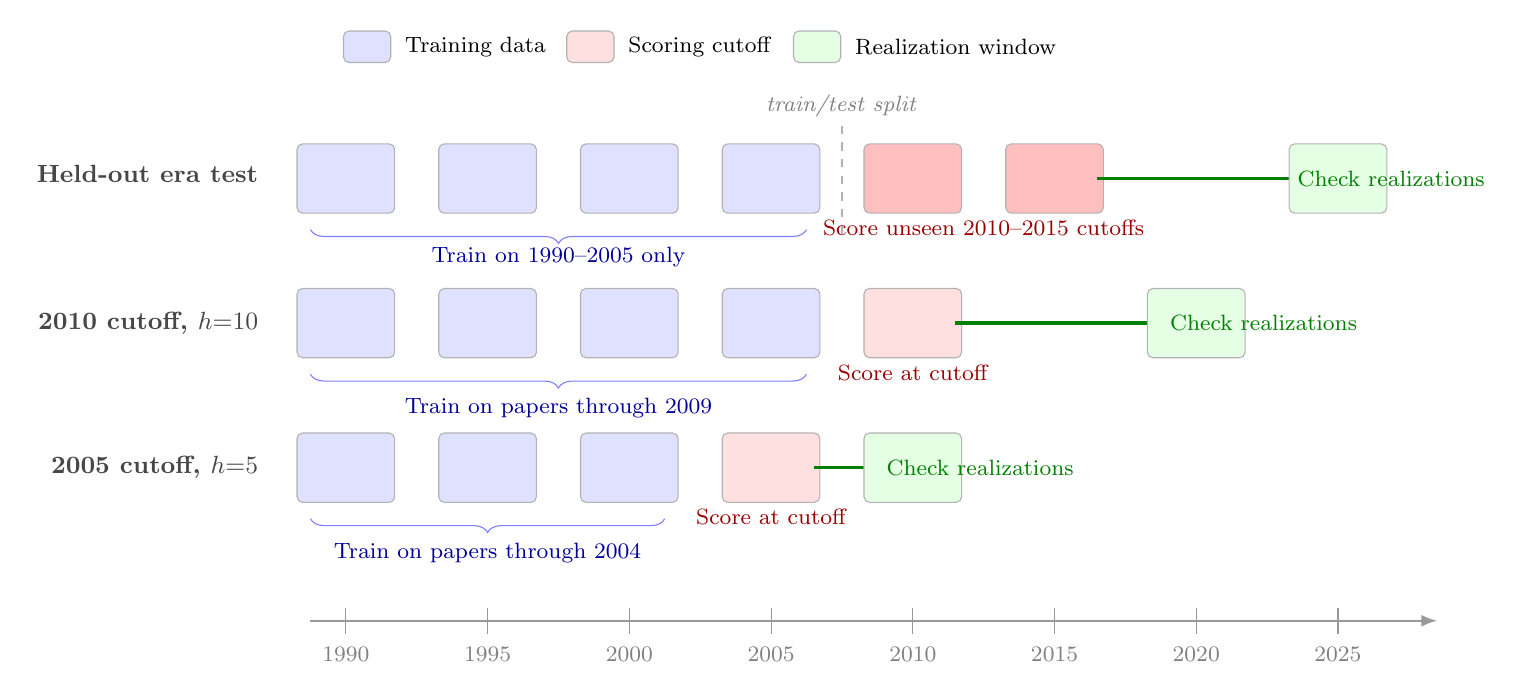
\begin{tikzpicture}[
    x=0.9cm, y=1.08cm,
    yearbox/.style={draw=black!30, rounded corners=2pt, minimum width=1.24cm, minimum height=0.88cm, font=\footnotesize, align=center},
    trainbox/.style={yearbox, fill=blue!12},
    evalbox/.style={yearbox, fill=red!12},
    horizonbox/.style={yearbox, fill=green!10},
    brace/.style={decorate, decoration={brace, amplitude=5pt, mirror}},
    annot/.style={font=\footnotesize, text=black!70},
    rowlabel/.style={font=\small\bfseries, text=black!72},
  ]
    \draw[-{Latex[length=2mm]}, thick, black!40] (-0.5,-0.3) -- (15.4,-0.3);
    \foreach \x/\yr in {0/1990, 2/1995, 4/2000, 6/2005, 8/2010, 10/2015, 12/2020, 14/2025} {
      \draw[black!40] (\x,-0.15) -- (\x,-0.45);
      \node[font=\footnotesize, text=black!50] at (\x,-0.7) {\yr};
    }
    \node[rowlabel, anchor=east] at (-1.1,1.5) {2005 cutoff, $h{=}5$};
    \foreach \x in {0,2,4} { \node[trainbox] at (\x,1.5) {}; }
    \node[evalbox] at (6,1.5) {};
    \draw[green!50!black, very thick, -{Latex[length=2mm]}] (6.6,1.5) -- (8.4,1.5);
    \node[horizonbox] at (8,1.5) {};
    \draw[brace, blue!50] (-0.5,0.9) -- (4.5,0.9);
    \node[font=\footnotesize, text=blue!60!black] at (2,0.5) {Train on papers through 2004};
    \node[font=\footnotesize, text=red!60!black] at (6,0.92) {Score at cutoff};
    \node[font=\footnotesize, text=green!50!black] at (8.95,1.5) {Check realizations};
    \node[rowlabel, anchor=east] at (-1.1,3.2) {2010 cutoff, $h{=}10$};
    \foreach \x in {0,2,4,6} { \node[trainbox] at (\x,3.2) {}; }
    \node[evalbox] at (8,3.2) {};
    \draw[green!50!black, very thick, -{Latex[length=2mm]}] (8.6,3.2) -- (12.4,3.2);
    \node[horizonbox] at (12,3.2) {};
    \draw[brace, blue!50] (-0.5,2.6) -- (6.5,2.6);
    \node[font=\footnotesize, text=blue!60!black] at (3,2.2) {Train on papers through 2009};
    \node[font=\footnotesize, text=red!60!black] at (8,2.62) {Score at cutoff};
    \node[font=\footnotesize, text=green!50!black] at (12.95,3.2) {Check realizations};
    \node[rowlabel, anchor=east] at (-1.1,4.95) {Held-out era test};
    \foreach \x in {0,2,4,6} { \node[trainbox] at (\x,4.9) {}; }
    \draw[black!30, thick, dashed] (7.0,4.25) -- (7.0,5.55);
    \node[evalbox, fill=red!25] at (8,4.9) {};
    \node[evalbox, fill=red!25] at (10,4.9) {};
    \draw[green!50!black, very thick, -{Latex[length=2mm]}] (10.6,4.9) -- (14.0,4.9);
    \node[horizonbox] at (14,4.9) {};
    \draw[brace, blue!50] (-0.5,4.3) -- (6.5,4.3);
    \node[font=\footnotesize, text=blue!60!black] at (3,3.98) {Train on 1990--2005 only};
    \node[font=\footnotesize, text=black!50] at (7.0,5.75) {\textit{train/test split}};
    \node[font=\footnotesize, text=red!60!black] at (9,4.32) {Score unseen 2010--2015 cutoffs};
    \node[font=\footnotesize, text=green!50!black] at (14.75,4.9) {Check realizations};
    \node[trainbox, minimum width=0.6cm, minimum height=0.4cm] at (0.3,6.45) {};
    \node[font=\footnotesize, anchor=west] at (0.7,6.45) {Training data};
    \node[evalbox, minimum width=0.6cm, minimum height=0.4cm] at (3.45,6.45) {};
    \node[font=\footnotesize, anchor=west] at (3.85,6.45) {Scoring cutoff};
    \node[horizonbox, minimum width=0.6cm, minimum height=0.4cm] at (6.65,6.45) {};
    \node[font=\footnotesize, anchor=west] at (7.05,6.45) {Realization window};
  \end{tikzpicture}
  }
  }
  \fignotes{This figure exists to show the paper's temporal discipline visually. At each cutoff, the graph uses only papers published before that date (blue). Candidates are scored at the cutoff (red), and realizations are checked over the horizon window (green). The bottom row shows the held-out era test from Appendix~\ref{app:temporal-generalization}: train on 1990--2005 and evaluate on the unseen 2010--2015 era.}
\end{figure}

\paragraph{Benchmark objects and metrics.}
The paper keeps two dated historical objects side by side. In path-to-direct, a local path
already exists and the later event is the first appearance of the direct link. In
direct-to-path, a direct relation already exists and the later event is the first appearance
of a supporting path. \emph{Future links per 100 suggestions} is the shortlist hit rate:
Precision@\(K\), expressed per 100 suggestions so it stays comparable across reading
budgets. Recall@100 asks what share of all later realizations in that family appear in the
top 100. Mean reciprocal rank rewards putting later realizations nearer the top. These
measures should be compared within family first, and then across families with the
denominator difference in mind.

\paragraph{Preferential attachment as benchmark.} The first benchmark is a cumulative-advantage rule. It asks whether one can do well simply by following existing traffic in the graph. A candidate looks better when it joins two endpoints that already attract many links. The standard network name for that logic is \emph{preferential attachment}. In this paper it scores a candidate ordered pair by source out-degree times target in-degree:
\[
\mathrm{PA}(u,v)=d^{out}(u)\times d^{in}(v).
\]
It is a serious benchmark here, not a decorative one. Scientific attention is not allocated
by neutral exploration alone. Visible topics, familiar data, established methods, and a
larger installed literature often attract still more work. If a graph-based screen cannot
beat that rule, then future question choice is mostly a popularity process. The appendix
reports stronger transparent variants. The main text asks the simpler question of whether
graph structure adds screening value beyond cumulative advantage.\footnote{The label
``preferential attachment'' comes from the network-growth literature. In that literature,
nodes that already have many links are more likely to receive new ones
\citep{price1976general,barabasi1999emergence}. Readers who do not use the term can think of
it more simply as the graph analogue of cumulative advantage or a rich-get-richer process.
In a science setting, the same logic says that already visible papers, concepts, or topics
tend to attract still more connections. That is exactly why it is the right null in this
paper.}

\paragraph{Co-occurrence as a benchmark.} The second benchmark is a co-mention rule. It asks whether one really needs directed claim structure at all. Perhaps it is enough to know that two endpoint concepts appear together repeatedly in the same papers, even if one ignores direction, claim type, and local path structure. That is also a serious null in this setting. Many literatures are organized less by explicit causal direction than by repeated joint attention: topics, variables, and mechanisms that are often discussed together keep reappearing together. If that is the main force in the data, then a simple co-occurrence score should already recover much of what later gets studied. Much of the recent work on predicting future research connections takes exactly that route. Krenn and Zeilinger~\citeyearpar{krenn2020predicting} and Gu and Krenn~\citeyearpar{gu2025impact4cast}, for example, work with undirected co-occurrence, while related scientific-discovery systems often begin from co-mentioned entities or undirected knowledge links \citep{rzhetsky2015choosing,sourati2023accelerating}. That approach has clear advantages: it requires no extraction of causal direction or claim metadata, and it scales easily. The question here is whether the harder extraction of directed claim structure adds screening value beyond what co-mention alone delivers. I therefore include a co-occurrence baseline that scores each candidate pair by how many papers mention both endpoints, ignoring direction, claim type, and path structure.\footnote{I do not know of a clean economics paper that uses this exact co-occurrence rule as a prospective benchmark for open-question screening, so I do not force an economics citation here. In economics and adjacent bibliometric work, co-mention, co-citation, and keyword co-occurrence are more often used descriptively to map fields than prospectively to rank next questions. The role of the benchmark here is narrower: it asks whether repeated joint mention alone is already enough, or whether directed claim structure adds screening value on top of that.}

Preferential attachment is the cumulative-advantage null. Co-occurrence asks whether undirected co-mention is enough. The transparent graph score is the readable graph baseline. The learned reranker is the strongest graph-based screen on the same candidate set.

\paragraph{Fixed-budget retrieval.} The evaluation problem is not whether a useful question appears somewhere deep in a long ranking. It is whether useful questions appear in the first set a reader can plausibly inspect. Researchers do not read 5{,}000 candidates. Editors do not review 5{,}000 possibilities for a special issue. Funders do not investigate an unlimited menu of exploratory ideas. The relevant object is therefore a fixed reading budget: what does the graph deliver in the first 50, 100, or 500 suggestions that scarce attention can actually reach? That is why the paper emphasizes Recall@100, other fixed-budget shortlist measures, and frontier-style comparisons over larger \(K\). Those metrics are not a cosmetic presentation choice. They correspond to the real screening problem the paper is trying to inform.

\paragraph{Horizon choice.} The main horizons are 5, 10, and 15 years. Five years is a natural first window in economics because publication and diffusion are slow relative to many neighboring fields \citep{hadavand2024publishing}. But a five-year window is not enough to see many slower adjustments in topic, method, and citation uptake. Economics papers often keep accumulating attention over long citation life cycles, which is one reason to look beyond only the short run \citep{hamermesh2018citations}. Ten years therefore captures slower movement in questions that take time to propagate through papers, methods, and field conventions. Fifteen years remains empirically useful because many slower literatures are still only partly visible at shorter windows. Three years and twenty years are kept as appendix extensions, but the main benchmark comparison is now centered on 5, 10, and 15 years.

\section{Results}
\label{sec:results}

\subsection{Paired shortlist comparison}

The first comparison asks whether local structure adds anything beyond popularity. That is a
real test in this setting because research attention is path-dependent. Visible topics,
familiar data, and established methods tend to attract still more work. If that
cumulative-advantage process does most of the work, a popularity rule should already rank
future questions well. It does not. In both historical families, the transparent graph
score beats preferential attachment, and the learned reranker improves further.

The two families then diverge in form. Direct-to-path yields denser shortlists. In
plain language, a larger share of the top 100 suggestions later becomes part of the
published record. At \(h=5\), the learned reranker surfaces about 17.0 future links per 100
suggestions in direct-to-path, versus 10.7 in path-to-direct, which is equivalent to a
17.0\% versus 10.7\% shortlist hit rate. At \(h=10\), the comparison is 29.5 versus 21.2.
At \(h=15\), it is 41.2 versus 26.0. Path-to-direct instead captures more of the
later-realized stock and ranks it earlier on average. The learned reranker reaches
Recall@100 of 11.9, 15.5, and 15.3 across \(h=5,10,15\), versus 8.8, 9.6, and 7.7 in
direct-to-path (Figure~\ref{fig:main-benchmark} and
Table~\ref{tab:benchmark-summary-main}).

\begin{figure}[H]
  \caption{The two historical families are informative in different ways}
  \label{fig:main-benchmark}
  \centering
  \includegraphics[width=0.92\linewidth]{../outputs/paper/193_dual_family_main_pairing_field_overlap/dual_family_main_benchmark.pdf}
  \fignotes{Each row is one historical family and each column is one shortlist metric. Path-to-direct asks whether a locally supported direct relation later appears. Direct-to-path asks whether an existing direct relation later acquires a supporting path. Within each family, the transparent score beats preferential attachment and the learned reranker improves further. Across families, the comparison is not one-dimensional: direct-to-path delivers more later realizations per 100 suggestions, while path-to-direct has higher Recall@100 and MRR.}
\end{figure}

The top-100 shortlist recovers 10--15\% of the eventual realization stock from candidate pools that contain thousands of pairs. The graph helps, but it helps in different ways. In direct-to-path, the main gain is a denser flow of later realizations through the shortlist: Precision@100 rises. In path-to-direct, the main gain is bringing a larger share of the later-realized stock nearer the top of the ranking: Recall@100 and MRR rise.

The two families capture different forms of research progress and should not be collapsed into one generic score. Direct-to-path is most useful when an editor, researcher, or funder wants a sharp shortlist of claims that look paper-ready but still underworked. Path-to-direct is most useful when the task is to see which accepted claims are still structurally thin---where mechanism work is still missing. Much empirical economics moves from a reduced-form relation to channels, heterogeneity, and scope conditions, so direct-to-path is the more immediately readable family for most economists. But path-to-direct still matters: it closes missing direct claims that nearby support had already made plausible.

\subsection{Mechanism thickening versus direct closure}
\label{sec:path-evolution}

Which motion is more common? One is direct closure: a supporting path already exists at \(t-1\), the direct link does not, and that direct link later appears. The other is mechanism thickening: a direct link already exists at \(t-1\), but a supporting mediator path appears only later. The distinction separates two uses of research effort. Direct closure states a missing claim. Mechanism thickening explains, disciplines, or extends a claim the literature already treats as meaningful. Work on conservative search and declining disruption suggests that later work often develops accepted lines rather than replaces them with wholly new ones \citep{foster2015tradition,park2023disruptive}. I compare the two motions on the same dated length-2 graph structure (Figure~\ref{fig:candidate-schematic}).

\begin{figure}[t]
  \caption{Mechanism thickening is more common than direct closure}
  \label{fig:path-evolution}
  \centering
  
\includegraphics[width=0.88\linewidth]{path_evolution_comparison.png}
  \fignotes{``Path to direct'': a local path exists first and the direct link appears later. ``Direct to path'': the direct link exists first and a mediating path appears later. The figure exists to compare these two motions directly. Mechanism-deepening around existing claims dominates at all horizons.}
\end{figure}

The aggregate comparison is clear (Figure~\ref{fig:path-evolution}). Direct-to-path transitions dominate path-to-direct transitions in every cutoff-period block and at every horizon. The cleanest way to state this is in transition rates, because the eligible sets differ. At \(h=10\), the direct-to-path transition share rises from about 0.9\% in the 1990s to 4.3\% in the 2000s and 12.1\% in the 2010s---a roughly 12-fold increase over three decades---while the corresponding path-to-direct shares are about 0.3\%, 0.7\%, and 1.4\%.\footnote{These numbers use a length-2 definition of ``supporting path.'' Appendix~\ref{app:graph-evolution} reports the same rates under a length-3 definition (any three-hop chain $u \to w_1 \to w_2 \to v$). The direct-to-path share roughly doubles at every horizon under L3 (e.g., at $h=10$: 1.9\% $\to$ 10.3\% $\to$ 30.2\% across decades), while the path-to-direct share is diluted by the larger eligible set; the direct-to-path over path-to-direct ratio therefore strengthens, not weakens, when the path definition is broadened (Table~\ref{tab:path-evolution-L2-vs-L3}). The 12-fold figure in the text is the conservative length-2 version.}

The gap is large. Economics more often elaborates mechanisms around claims it already states
than closes a missing direct relation implied by nearby support. That is consistent with a
broader view of scientific change in which the literature more often thickens around
existing structure than opens wholly new direct connections
\citep{foster2015tradition,park2023disruptive}. The graph more often surfaces structured elaborations of accepted claims than missing direct
links between otherwise distant concepts. That helps explain why direct-to-path is the more
natural reader-facing object in economics: it lines up with a literature that often asks
not only whether a relation exists, but through what channel, under what conditions, and
with what supporting mechanism.

The pattern varies across the literature in economically interpretable ways. Adjacent journals are relatively more path-closure heavy than the core, but direct-to-path still dominates in both tiers. At \(h=5\), the share of realized transitions taking the path-to-direct form is about \(0.45\) in adjacent journals versus \(0.28\) in the core. Finance remains more direct-to-path heavy throughout. Figure~\ref{fig:path-source-mix} reports the journal-tier split. The asymmetry is therefore not an artefact of which journals are included in the core.

\begin{figure}[h]
  \caption{Adjacent journals close more path-implied links, but direct-to-path still dominates}
  \label{fig:path-source-mix}
  \centering
  
\includegraphics[width=0.90\linewidth]{path_transition_mix_by_source.png}
  \fignotes{This figure asks whether the transition mix differs by journal tier. It reports the share of realized path-related transitions taking the path-to-direct form by journal tier and horizon. Adjacent journals are consistently more path-closure heavy than the core, but direct-to-path remains the larger transition type in both tiers.}
\end{figure}

The paired evidence carries two lessons. In both historical families, graph structure
improves on popularity and the reranker improves further. The larger substantive point is
that much of scientific development takes the form of mechanism-deepening around existing
claims. The most useful next question is therefore often richer than a single missing edge.

\subsection{Reranked results in both families}

The learned reranker improves on the transparent score in both families. Keeping the
ontology, sample, and timing discipline fixed, it changes only how graph features are
weighted. The best configuration differs by family and horizon---the appendix reports the
full tuning table---but the direction is consistent: learned weighting moves more eventual
realizations toward the top of the shortlist. The improvement comes from combination
effects that the transparent fixed-weight score misses, not from additional data.

The transparent score remains useful alongside the reranker because it explains \emph{why}
a candidate looks promising in graph terms: path support, missingness relative to nearby
support, topology, and provenance. Table~\ref{tab:benchmark-summary-main} summarizes the
paired comparison.

\begin{table}[H]
  \caption{Paired benchmark summary for the two historical families}
  \label{tab:benchmark-summary-main}
  \centering
  \scriptsize
  \input{../outputs/paper/193_dual_family_main_pairing_field_overlap/dual_family_main_benchmark_table.tex}
  \fignotes{Each row reports one family-model combination averaged across the 1990--2015 cutoff grid. Columns are grouped by metric, with the three main horizons nested underneath. Future links per 100 suggestions is the shortlist hit rate, that is, Precision@100 expressed in percent. Recall@100 is the share of all later realizations in that family captured in the top 100. Mean reciprocal rank rewards putting later realizations nearer the top. The table shows the same pattern as Figure~\ref{fig:main-benchmark}: the graph beats preferential attachment in both families, the learned reranker improves further, and the two families remain substantively different rather than collapsing to one ranking problem.}
\end{table}

The paired shortlist comparison already shows that graph structure adds screening value
beyond popularity in both historical families. The reranker shows that the same candidate
universe can be ordered better still. Additional paired extensions, including the current
frontier and broader reading budgets, are therefore follow-on checks rather than the main
claim (Appendix~\ref{app:paired-family-extensions} and
Appendix~\ref{app:paired-budget-extensions}). The paired budget comparison adds one
practical lesson: path-to-direct is sharper when the reader wants a very short shortlist,
while direct-to-path becomes more useful once the reader is willing to inspect a broader
set of candidates (Appendix~\ref{app:paired-budget-extensions}).

\paragraph{What the reranker loads on.}
A grouped Shapley decomposition (Appendix~\ref{app:reranker-design}) separates two things the reranker does. It loads \emph{positively} on directed causal degree, recency, and evidence quality: pairs whose endpoints are central in the causal subgraph, have been the subject of recent research, and draw on well-evidenced concepts. It loads \emph{negatively} on broad support-graph popularity: once directed causal degree and recency are controlled for, being a well-connected concept in the wider support graph reduces the predicted probability of realization. In plain terms, the model identifies concept pairs whose recent and causally central activity outpaces their long-run popularity. That is the opposite of cumulative advantage, and the decomposition is stable across logistic and tree-based model families (Figure~\ref{fig:grouped-shap}).

\section{Discussion and Extensions}
\label{sec:discussion}

These results speak to a structural feature of the economics literature, not merely to the
performance of a ranking algorithm. At each historical cutoff, the graph stores the
directional accumulation of what the literature has already asserted and what it has
conspicuously left unsaid. When that structure predicts later publication at rates far above
the popularity baseline, it means past claims carry systematic information about where the
next ones will go. The asymmetry between the two families is equally informative. The
literature more often extends accepted claims through new mechanisms than it closes locally
implied direct relations---a pattern that is stable across eras and horizons. A screening
tool calibrated on such a literature will surface a larger share of mechanism-thickening
candidates: not because the algorithm favors them, but because that is the shape of
research progress in economics.

\paragraph{What the distinction means.}
The two historical objects capture different parts of research progress. Direct closure is
the case where nearby support already points toward a relation that later becomes explicit.
Mechanism thickening is the case where a known relation later acquires a clearer channel.
Economists care about both, but they help in different ways. Direct-closure questions are
useful when a researcher, editor, or funder wants a sharper shortlist of claims that look
paper-ready but still underworked. Mechanism-thickening questions are useful when the task
is to see where an accepted result is still structurally thin. The historical record says
the second move is more common. A useful screening tool should therefore not only point
toward underworked direct relations. It should also help identify where an accepted claim
still lacks a convincing mechanism.

\paragraph{Why to trust the pattern.}
One reason to take that result seriously is that it does not rest on one fragile ranking
rule. The main paired comparison survives the move from a transparent score to a learned
reranker, and the reranker carries forward to later vintages that were not used for model
selection (Figure~\ref{fig:temporal-generalization-main}). The appendices show the same
discipline more broadly: the extraction layer is auditable, the directed claim graph is not
just undirected co-mention in disguise, and the natural extensions confirm rather than
reverse the main pattern.\footnote{The held-out temporal test is reported in
Appendix~\ref{app:temporal-generalization}. The author-positioning null result is discussed
in Appendix~\ref{app:reranker-design}. Credibility and stability audits are collected in
Appendix~\ref{app:credibility-audit}.}

\begin{figure}[t]
  \caption{The reranker generalizes forward in time}
  \label{fig:temporal-generalization-main}
  \centering
  \includegraphics[width=0.90\linewidth]{temporal_generalization.png}
  \fignotes{For each main horizon, the reranker is selected using only 1990--2005 cutoff cells and then evaluated on the fully held-out 2010--2015 era. Labels report the reranker's absolute \(P@100\) gap relative to preferential attachment. The held-out gap is larger than the earlier training-era gap at both \(h=5\) and \(h=10\). Full results in Appendix Table~\ref{tab:temporal-generalization}.}
\end{figure}

\paragraph{Where the graph helps.}
Two broader implications follow. First, the graph does not add the most value where the
literature is maximally thin. The appendix regime splits show that its comparative advantage is
larger where some usable local structure already exists. So this is not a machine for
discovering the most remote idea in the graph. It is a screening device for the large middle
of the literature, where there is enough nearby evidence to make a question legible but
still enough missing structure that attention can be reallocated productively. Second, if
the literature usually moves by thickening mechanisms around existing claims, then one
useful role for computational tools is not open-ended idea generation. It is to help
economists see where an accepted relation is still structurally underexplained.

\paragraph{Benchmark event and surfaced question.}
Keeping the benchmark and the reader-facing question separate follows from that logic. A
dated graph event is useful because it can be tested prospectively. A surfaced question is
useful because it can be read, argued over, and discarded if it is uninteresting. The
historical benchmark gives discipline. The surfaced object gives the tool practical value.
Supplementary human and LLM usefulness checks remain secondary for that reason: they help
assess whether the surfaced questions are readable, but they do not replace the historical
evidence.\footnote{Appendix~\ref{app:current-usefulness} reports a small blinded human
exercise and a larger appendix LLM screen. Both are useful as screening checks, not as
substitutes for the historical benchmark.}

\paragraph{Budget interpretation.}
The budget results sharpen that interpretation. Scarce attention is not only an individual
researcher's problem. It is also an editorial, funding, and field-level problem. On that
margin, the two historical families do not play the same role. Path-to-direct is more
useful for triage: it concentrates more realized direct closures near the top of a short
list. Direct-to-path is more useful for exploration: once the reading budget widens, it
recovers a much broader share of the future mechanism literature. That is the relevant
object when the problem is to see where an accepted relation is still underexplained rather
than merely underclaimed.

These budget results also connect the paper to a broader literature on how science allocates
attention \citep{jones2009burden,bloom2020ideas,azoulay2011incentives,foster2015tradition,packalen2020stagnation}.
That literature emphasizes the rising burden of reaching the frontier and the institutional
tilt toward safer, more familiar directions. The present paper does not solve that problem
at the level of incentives. But it does speak to scientific method in a narrower way: under
severe screening constraints, a useful method is one that moves more plausible questions
into the stage where economists, editors, and funders can exercise judgment. The graph is
not a replacement for judgment. It is a disciplined way to widen the agenda that reaches
judgment.

\paragraph{Bundle uptake.}
Later papers could in principle realize a bundle of predicted edges rather than one. Work in science-of-science has emphasized that
novel contributions often recombine nearby ingredients rather than arriving as isolated
moves \citep{uzzi2013atypical,foster2015tradition,fortunato2018science}. The bundle-uptake
analysis in Appendix~\ref{app:bundle-uptake} suggests that the dominant downstream object in
this setting is still a single paper-shaped question: only about five percent of realizing
papers take up more than one historically predicted edge, and mixed-family bundles are very
rare. But when multi-edge uptake does occur, it is strongly local in graph space. That
result helps interpret the budget evidence. The wider-budget advantage of
\emph{direct-to-path} seems to come mainly from broader coverage across many separate
papers, not from a large number of later papers each realizing multiple predicted edges across both families.

\paragraph{Extensions.}
Two extensions are most worth developing. The first is to test whether the mechanism-thickening asymmetry is specific to economics or a broader feature of cumulative science. Applying the same walk-forward benchmark to sociology, political science, and psychology would reveal whether directed claim graphs in other social sciences show the same imbalance between mechanism elaboration and direct closure. The second is dynamic concept activation. The current benchmark holds the active concept set fixed at each cutoff, but some of the highest-impact work introduces entirely new nodes. A model that predicts when a dormant concept pair becomes active---rather than when a missing edge closes---would complement the missing-link design and speak more directly to radical novelty.

This paper provides a prospectively testable historical design, a readable surfaced object,
and an honest comparison with the cumulative-advantage null.
That is enough to establish that the nearby structure of the literature carries screening
information that popularity alone misses. If ideas are harder to find and downstream
research tasks are getting cheaper, the value of better upstream screening rises.
Economics should not decide what to work on next only through popularity and familiarity.
The graph offers a structured way to widen the set of questions that reaches the judgment
stage---not to replace judgment, but to give it more to work with.

\appendix
\clearpage

\begin{titlepage}
  \centering
  \vspace*{\fill}
  {\Huge\bfseries Appendix\par}
  \vspace{0.75em}
  {\Large What Should Economics Ask Next?\par}
  \vspace*{\fill}
\end{titlepage}

\section{Guide to the Appendix}
\label{app:appendix-guide}

The appendix has five jobs. First, it documents how the graph is built from title and
abstract text. Second, it records the benchmark tables and reranker detail that support the
main text without carrying its argument. Third, it collects paired and family-specific
extensions that are useful once the main comparison is clear. Fourth, it reports audit and
presentation checks on the graph and on the surfaced questions. Fifth, it adds a short set
of supplementary analyses on how later papers realize predicted ideas and which kinds of
teams move toward them. The main text remains narrow: paired shortlist results first,
then the path-versus-mechanism result, then the confirmatory reranker comparison.

\begin{table}[t]
  \caption{Positioning relative to closest comparable work}
  \label{tab:positioning}
  \centering
  \small
  \begin{tabular}{L{0.14\linewidth}L{0.15\linewidth}L{0.17\linewidth}L{0.23\linewidth}L{0.16\linewidth}}
    \toprule
    & This paper & Impact4Cast & Sourati et al. & Tong et al. \\
    \midrule
    Domain & Economics & All sciences & Biomedicine & Psychology \\
    Edge type & Directed causal & Co-occurrence & Co-occurrence & Causal \\
    Corpus & 242{,}595 papers & 2.4M papers & Varies & 43{,}312 papers \\
    Main null & Preferential attachment & ML baselines & Content-only & TransE \\
    Temporal eval & Prospective walk-forward & Holdout & Holdout & None \\
    Human eval & Appendix checks & No & No & Yes \\
    \bottomrule
  \end{tabular}
  \fignotes{Impact4Cast: Gu and Krenn~\citeyearpar{gu2025impact4cast}. Sourati et al.: Sourati et al.~\citeyearpar{sourati2023accelerating}. Tong et al.: Tong et al.~\citeyearpar{tong2024automating}. The table compares the closest systems along the dimensions most relevant for this paper: domain, edge type, scale, main null, temporal design, and whether any human check is reported.}
\end{table}

\input{appendix_paired_family_extensions.tex}
\input{appendix_paired_budget_extensions.tex}
\input{appendix_direct_closure_extensions.tex}

\section{Paper-local Extraction}
\label{app:extraction-protocol}

This appendix documents how title-and-abstract text is turned into the paper-local graphs
used in the benchmark. The core object is simple: one paper becomes one local graph of
concepts and relations. Garg and Fetzer~\citeyearpar{gargfetzer2025causal} show that this is
feasible for economics papers. The present paper uses the same starting point for a
different downstream purpose: a reusable graph that can support missing-link construction,
candidate ranking, and later concept matching across papers.

Three design choices matter most. First, the schema includes undirected relations, because
contextual support is useful even when the headline task is directed causal emergence.
Second, the schema separates the paper's \emph{causal presentation} from the
\emph{evidence method} used to support a relation. A paper can speak causally while using a
weak design, or it can use a stronger design while describing the finding cautiously.
Third, local scope qualifiers are stored separately from the node label whenever possible,
so that later normalization can target concept identity rather than local sample wording.

\subsection{Extraction prompts}

The benchmark uses a fixed system prompt and a minimal user prompt template. They are reproduced exactly below for auditability.

\paragraph{System prompt.}
  \promptfile{../prompts/frontiergraph_extraction/system_prompt.md}

\paragraph{User prompt template.}
  \promptfile{../prompts/frontiergraph_extraction/user_prompt_template.md}

\subsection{Extraction schema}

The model returns a paper-local graph with \texttt{nodes} and \texttt{edges}. The underlying output is JSON. Tables~\ref{tab:node-schema} and~\ref{tab:edge-schema} restate the fields in reader-facing labels.
\begingroup
\scriptsize
\begin{longtable}{L{0.22\linewidth}L{0.16\linewidth}L{0.27\linewidth}L{0.23\linewidth}}
  \caption{Schema for paper-local nodes}
  \label{tab:node-schema}\\
  \toprule
  Field & Allowed values / type & Meaning & Why it exists downstream \\
  \midrule
  \endfirsthead
  \toprule
  Field & Allowed values / type & Meaning & Why it exists downstream \\
  \midrule
  \endhead
  Node identifier (\texttt{node\_id}) & string & Paper-local identifier such as \texttt{n1}. & Needed so edges can reuse the same local concept deterministically within a paper. \\
  Concept label (\texttt{label}) & short string & Concise concept label grounded in the title/abstract. & Becomes the base string passed into normalization and ontology mapping. \\
  Surface forms (\texttt{surface\_forms}) & array of strings & Distinct surface mentions in the title/abstract that refer to the same local concept. & Preserves within-paper synonymy without forcing global canonicalization at extraction time. \\
  Unit of analysis\\(\texttt{study\_context.}\\\texttt{unit\_of\_analysis}) & array of enumerated strings & Explicit unit of analysis linked to the node, if stated. & Keeps sample and scope off the concept label while preserving paper-local context. \\
  Start year\\(\texttt{study\_context.}\\\texttt{start\_year}) & array of integers & Explicit start years if stated. & Preserves local scope without creating separate concept nodes for years. \\
  End year\\(\texttt{study\_context.}\\\texttt{end\_year}) & array of integers & Explicit end years if stated. & Same reason as start year. \\
  Countries\\(\texttt{study\_context.}\\\texttt{countries}) & array of strings & Explicit countries if stated. & Preserves local setting without baking geography into concept identity unless essential. \\
  Context note\\(\texttt{study\_context.}\\\texttt{context\_note}) & string & Residual local scope text such as ``older workers'' or ``rural counties''. & Retains paper-local nuance for audit and display while leaving the node label concept-level. \\
  \bottomrule
\end{longtable}

\begin{longtable}{L{0.22\linewidth}L{0.18\linewidth}L{0.25\linewidth}L{0.23\linewidth}}
  \caption{Schema for paper-local edges}
  \label{tab:edge-schema}\\
  \toprule
  Field & Allowed values / type & Meaning & Why it exists downstream \\
  \midrule
  \endfirsthead
  \toprule
  Field & Allowed values / type & Meaning & Why it exists downstream \\
  \midrule
  \endhead
  Edge identifier (\texttt{edge\_id}) & string & Paper-local identifier such as \texttt{e1}. & Stable local relation key. \\
  Source and target nodes\\(\texttt{source\_node\_id}, \texttt{target\_node\_id}) & strings & Local source and target node references. & Connect extracted relations back to the paper-local node inventory. \\
  Directionality (\texttt{directionality}) & directed / undirected & Whether the text presents the relation directionally. & Determines whether the downstream graph stores an ordered link or an undirected contextual pair. \\
  Relationship type (\texttt{relationship\_type}) & effect / association / prediction / difference / other & Coarse semantic type of the relation. & Supports later filtering and audit of what kind of relation is being surfaced. \\
  Causal presentation (\texttt{causal\_presentation}) & explicit\_causal / implicit\_causal / noncausal / unclear & How the paper \emph{describes} the relation. & Separates language from design quality; useful for credibility audits and task splitting. \\
  Argument role (\texttt{edge\_role}) & main\_effect / mechanism / heterogeneity / descriptive\_pattern / background / robustness / other & Role of the relation inside the paper's argument. & Distinguishes central claims from channels, subgroup effects, and background statements. \\
  Claim status (\texttt{claim\_status}) & effect\_present / no\_effect / mixed\_or\_ambiguous / conditional\_effect / question\_only / other & What result the paper reports for the relation. & Prevents question-only edges from being treated as equivalent to reported positive results. \\
  Explicitness (\texttt{explicitness}) & result\_only / question\_only / question\_and\_result / background\_claim / implied & How explicitly the relation is framed in text. & Useful for separating central reported findings from implied or motivating claims. \\
  Condition or scope\\(\texttt{condition\_or\_scope\_text}) & string & Edge-level scope or subgroup qualifier. & Keeps conditional language attached to the relation rather than the node. \\
  Claim text (\texttt{claim\_text}) & string & Short normalized relation text. & Audit-friendly summary of the extracted edge. \\
  Evidence text (\texttt{evidence\_text}) & string & Short supporting excerpt or close paraphrase from the title/abstract. & Makes the edge inspectable in the public tool and in manual audits. \\
  Direction of effect (\texttt{sign}) & increase / decrease / no\_effect / ambiguous / NA & Reported sign of the relation when stated. & Supports later descriptive summaries and credibility splits. \\
  Effect size (\texttt{effect\_size}) & string & Reported magnitude if stated. & Retained for completeness and future extensions. \\
  Statistical significance (\texttt{statistical\_significance}) & significant / not\_significant / mixed\_or\_ambiguous / not\_reported / NA & Significance status stated in text. & Keeps reported evidence strength distinct from sign or design. \\
  Evidence method (\texttt{evidence\_method}) & enumerated method family & Main method family named or implied in the abstract. & Determines whether a relation enters the graph as directed causal or undirected contextual support. \\
  Other method description\\(\texttt{evidence\_method\_other\_description}) & string & Free-text description when method is \texttt{other}. & Preserves method specificity without exploding the method taxonomy. \\
  Nature of evidence (\texttt{nature\_of\_evidence}) & quantitative / qualitative / mixed\_methods / theoretical\_or\_conceptual / simulation / review\_or\_commentary / NA & Broad evidence type. & Helps later distinguish theory, empirical, and simulation-heavy slices. \\
  Uses data (\texttt{uses\_data}) & boolean & Whether the edge is supported by data use. & Simple empirical-versus-theory indicator. \\
  Exogenous variation source\\(\texttt{sources\_of\_exogenous\_variation}) & string & Explicit source of exogenous variation if named. & Reserved for future credibility-weighting extensions. \\
  Tentativeness (\texttt{tentativeness}) & certain / tentative / mixed\_or\_qualified / unclear & How assertive the language is. & Keeps cautious claims distinct from strong declarative ones. \\
  \bottomrule
\end{longtable}
\endgroup

\subsection{Extraction design choices}

\paragraph{Paper-local node reuse.} The model is asked to reuse the same local node whenever the same concept genuinely recurs within a paper. That choice matters because downstream graph construction depends on whether a path inside one paper reuses a local concept consistently. If each mention were given a fresh node, the later concept graph would inherit spurious fragmentation before normalization even begins.

\paragraph{No transitive closure.} The prompt explicitly forbids the model from creating \(A \rightarrow C\) when the text only states \(A \rightarrow B\) and \(B \rightarrow C\). This is crucial for the benchmark. Missing direct links are the object of interest. If extraction itself created transitive closure, the benchmark would mechanically erase many of the very candidates it later wants to rank.

\paragraph{Directed versus undirected storage.} The extraction schema stores one undirected relation using the first-mentioned concept as a storage convention, rather than duplicating it as two directed edges. This keeps contextual support distinct from directionally stated claims and avoids turning association language into artificial causal direction.

\paragraph{Keeping scope off the node label.} Country, year, subgroup, and sample qualifiers are stored in dedicated context fields whenever possible. This is a normalization choice made early. A benchmark that ranks missing links between concepts needs concept identity to remain as stable as possible across papers. Local scope still matters for audit and interpretation, but it should not automatically become part of the canonical node label.

\paragraph{Separating causal presentation from evidence method.} A paper can talk causally without using a strong design, and it can use a stronger design while describing the result more cautiously. Keeping these separate is what later allows the benchmark to define directed causal candidates by method while still auditing how papers describe those relations.

\paragraph{Separating claim status, explicitness, tentativeness, and edge role.} These fields overlap in plain language but do different jobs downstream. Claim status records whether a finding is present, absent, mixed, or only posed as a question. Explicitness records whether the relation is stated as a result, a question, background, or only implied. Tentativeness records how strongly the paper speaks. Edge role records whether the relation is the main effect, a mechanism, heterogeneity, or something else. The benchmark and public tool both become much less legible if these distinctions are collapsed into one generic confidence flag.

\paragraph{Reproducibility.} The prompts, schema files, extraction scripts, ontology pipeline, and paper-generation code are available at \repoURL.

\section{Normalization and Ontology}
\label{app:node-normalization}

Node normalization is central because candidate generation, path counts, and missingness all
depend on node identity. Paper-level concept strings vary in wording, scope, and
granularity, so node definition cannot be treated as a secondary detail.

\subsection{Why open-world normalization}

Garg and Fetzer~\citeyearpar{gargfetzer2025causal} use paper-local extracted objects for a
different downstream task. The present paper asks a more node-sensitive question. Here the
downstream object is a reusable concept graph in which a candidate next paper is a missing
link between \emph{specific concepts}. In that setting, concept identity cannot be handled
at a broad field level. The benchmark needs to preserve distinctions such as public debt
versus public investment, or monetary policy versus energy consumption.

The difficulty is that the extraction layer and the ontology layer speak slightly different
languages. Extraction produces paper-local phrases such as ``gdp per capita'',
``renewable energy consumption'', or ``financial frictions''. The ontology contains more
canonical labels. A useful grounding system therefore cannot be binary. If it only keeps
exact or near-exact matches, it overselects the cleanest vocabulary and risks dropping real
economics concepts from the graph. If it accepts every nearest neighbor, it creates false
precision. The frozen ontology design used here is therefore \emph{open-world}: it allows
exact grounding, broader grounding, lower-confidence candidate bands, and unresolved labels
that remain visible for later review rather than disappearing from the graph.

\begin{figure}[t]
  \caption{Node normalization and concept matching}
  \label{fig:normalization-flow}
  \centering
  \resizebox{0.94\linewidth}{!}{%
  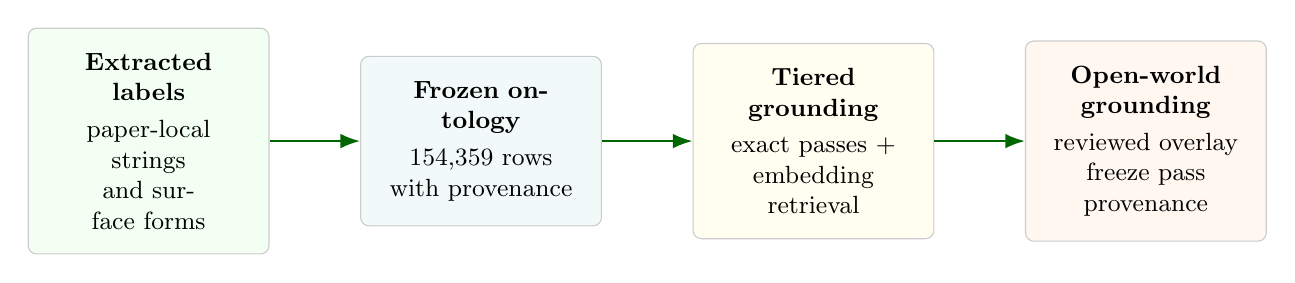
\begin{tikzpicture}[
    node distance=1.15cm,
    box1/.style={draw=black!20, rounded corners=3pt, fill=green!5, text width=0.20\linewidth, minimum height=1.75cm, inner sep=9pt, align=center, font=\small},
    box2/.style={draw=black!20, rounded corners=3pt, fill=teal!5, text width=0.20\linewidth, minimum height=1.75cm, inner sep=9pt, align=center, font=\small},
    box3/.style={draw=black!20, rounded corners=3pt, fill=yellow!6, text width=0.20\linewidth, minimum height=1.75cm, inner sep=9pt, align=center, font=\small},
    box4/.style={draw=black!20, rounded corners=3pt, fill=orange!6, text width=0.20\linewidth, minimum height=1.75cm, inner sep=9pt, align=center, font=\small},
    arr/.style={-{Latex[length=2.5mm]}, thick, draw=green!40!black}
  ]
    \node[box1] (raw) {\textbf{Extracted labels}\\[0.25em]paper-local strings\\and surface forms};
    \node[box2, right=of raw] (heads) {\textbf{Frozen ontology}\\[0.25em]154{,}359 rows\\with provenance};
    \node[box3, right=of heads] (maps) {\textbf{Tiered grounding}\\[0.25em]exact passes +\\embedding retrieval};
    \node[box4, right=of maps] (graph) {\textbf{Open-world grounding}\\[0.25em]reviewed overlay\\freeze pass\\provenance};
    \draw[arr] (raw) -- (heads);
    \draw[arr] (heads) -- (maps);
    \draw[arr] (maps) -- (graph);
  \end{tikzpicture}
  }
  \fignotes{This figure summarizes the frozen ontology grounding pipeline used in the benchmark. Paper-local labels are matched to a structured-source ontology by exact label and surface-form passes first, then by embedding retrieval. Lower-confidence labels are not simply dropped: broader grounding is allowed, reviewed outcomes remain explicit, and unresolved labels remain visible with provenance.}
\end{figure}

\subsection{Implemented pipeline}

The ontology build proceeds in five stages (Figure~\ref{fig:normalization-flow};
Table~\ref{tab:mapping-stages} summarizes each stage).

\paragraph{Ontology assembly.} The frozen ontology baseline starts from five structured
source families rather than from the paper corpus alone. JEL provides a controlled
economics taxonomy. Wikidata adds identifier-grounded concepts and aliases. OpenAlex topics
and keywords add current research vocabulary. An economics-filtered Wikipedia crawl adds
fine-grained named concepts, policies, instruments, and episodes that appear in extraction
labels but are absent from the structured sources. A small reviewed family layer is also
carried forward. The resulting baseline contains 154{,}359 rows.

\paragraph{Label inventory and exact grounding.} The extraction corpus contributes
1{,}389{,}907 unique normalized labels from 242{,}595 papers. Mapping begins with exact
matches on the extracted label itself and then exact matches on stored surface forms,
including stripped parenthetical variants. These deterministic passes solve the easy cases
without using embeddings.

\paragraph{Embedding retrieval and confidence bands.} Labels that remain unresolved after
the exact passes are embedded and searched against the ontology with FAISS nearest-neighbour
retrieval. The rank-1, rank-2, and rank-3 ontology candidates are stored for audit. The
resulting grounding is tiered rather than binary: \texttt{linked} for scores at or above
0.85, \texttt{soft} for 0.75--0.85, \texttt{candidate} for 0.65--0.75,
\texttt{rescue} for 0.50--0.65, and \texttt{unresolved} below 0.50. Across the
1{,}389{,}907 normalized extracted labels, 316{,}292 unique labels clear the primary 0.75
threshold before any reviewed open-world layer is applied. Lower-confidence bands remain
visible rather than being silently dropped.

\paragraph{Reviewed open-world grounding.} Lower-confidence labels are then audited with an
overlay-first review pass. That layer keeps broader attachment to an existing concept, alias
addition, proposed concept-family promotion, explicit rejection, and unresolved outcomes
separate rather than forcing everything into one nearest-neighbour merge. Broader grounding
is allowed when the ontology only contains a more general concept. That is intentional. For
example, grounding ``gdp per capita'' to the broader concept ``GDP'' can be more
informative than dropping the label entirely. Raw labels and raw edges are preserved
throughout, so ontology weakness does not mechanically create spurious graph gaps.

\paragraph{Freeze pass and reviewed hierarchy.} The conservative freeze turns that review
work into a stable paper-facing ontology layer. It preserves the raw label, source, parent
label, and root label fields, adds cleaned display labels where needed, and records
reviewed effective-parent and effective-root overlays. The key design choice is conservative
rather than exhaustive: the freeze accepts only a small number of additional duplicate
merges and leaves the remaining too-broad or unresolved cases explicit rather than silently
patching them.

\begin{table}[t]
  \caption{Stages of the ontology pipeline}
  \label{tab:mapping-stages}
  \centering
  \begin{tabular}{L{0.16\linewidth}L{0.34\linewidth}L{0.38\linewidth}}
    \toprule
    Stage & What it does & Why it is needed \\
    \midrule
    Ontology assembly & Combines JEL, Wikidata, OpenAlex topics, OpenAlex keywords, and filtered Wikipedia into one deduplicated concept inventory. & Gives the graph a broad structured concept vocabulary rather than relying on a single taxonomy. \\
    Exact grounding & Applies exact label, exact surface-form, and stripped-parenthesis matches. & Solves easy cases deterministically before any embedding step. \\
    Embedding grounding & Uses nearest-neighbour embedding retrieval and stores rank-1 to rank-3 candidates. & Grounds the harder middle of the label distribution while keeping retrieval provenance. \\
    Reviewed open-world grounding & Keeps broader attachments, alias additions, proposed family rows, explicit rejections, and unresolved outcomes separate. & Prevents the ontology tail from being treated as either fully trusted or silently dropped. \\
    Freeze pass & Adds cleaned display labels, reviewed hierarchy overlays, and conservative duplicate review while preserving raw fields. & Stabilizes the paper-facing ontology baseline without rewriting source truth. \\
    \bottomrule
  \end{tabular}
  \fignotes{This is a process table, not an estimation table. Each row is one stage in the ontology pipeline that turns paper-local labels into the concept vocabulary used for candidate generation and benchmarking. The main distinction is between automatic grounding steps, which handle exact or embedding-based matches, and reviewed open-world steps, which keep lower-confidence cases visible instead of silently dropping them.}
\end{table}

\subsection{Preserving the raw graph and tiering the ontology}

The key choice is not to let ontology confidence determine which literatures count as candidate-generating. If low-confidence labels were simply dropped, the benchmark would overselect the cleanest, most repetitive, and most canonical concept strings. It would also risk creating spurious novelty whenever a real but underrepresented concept failed to receive a clean ontology attachment. The solution used here is therefore to preserve the raw extraction graph while treating ontology grounding as a tiered interpretive layer. High-confidence grounded labels can be aggregated immediately. Lower-confidence labels can still receive broader grounding or reviewed unresolved status. The freeze then stabilizes the paper-facing ontology layer without pretending the remaining tail has been solved.

\input{appendix_graph_evolution.tex}

\section{Benchmark Design and Significance}
\label{app:benchmark-details}

This appendix records the sample counts, benchmark tables, and significance summaries behind
the main comparison. It does not introduce a second empirical object. Table~\ref{tab:corpus-summary}
summarizes the two most important transitions: from selected journal papers to papers with
extracted edges, and then from raw extracted edges to normalized evaluation links. The
frozen ontology baseline is reported separately because the ontology inventory and the active
benchmark graph are distinct objects.

\begin{table}[h]
  \caption{Corpus and normalization summary}
  \label{tab:corpus-summary}
  \centering
  \begin{tabular}{lr}
    \toprule
    Quantity & Count \\
    \midrule
    Selected journal papers & 242{,}595 \\
    Papers with extracted edges & 230{,}929 \\
    Raw extracted edges & 1{,}443{,}407 \\
    Normalized benchmark papers & 230{,}479 \\
    Frozen ontology baseline concepts & 154{,}359 \\
    Directed causal rows & 89{,}737 \\
    Undirected contextual rows & 1{,}181{,}277 \\
    Total normalized links & 1{,}271{,}014 \\
    \bottomrule
  \end{tabular}
  \fignotes{This table reports the sample counts behind the benchmark. The rows move from the selected journal corpus to papers with extracted relations, then to the normalized graph used for candidate generation and evaluation. ``Frozen ontology baseline concepts'' refers to the paper-facing concept inventory after the reviewed freeze pass. ``Total normalized links'' is the active graph edge count used in the benchmark.}
\end{table}

The stricter identified-causal-claim layer is retained as a nested continuity
benchmark. I do not use it as the main task, because it is much sparser than
the broader causal-claim anchor used in the main text. But it is still useful as a
conservative reference object, especially for readers who want continuity with the
credibility-focused specification. Table~\ref{tab:strict-main-benchmark} reports that
continuity benchmark, and Table~\ref{tab:strict-significance} reports the paired bootstrap
comparison against preferential attachment on the same stricter layer.

\begin{table}[h]
  \caption{Continuity benchmark on the identified-causal-claim layer}
  \label{tab:strict-main-benchmark}
  \centering
  \begin{tabular}{lccc}
    \toprule
    Metric & \(h=5\) & \(h=10\) & \(h=15\) \\
    \midrule
    Recall@100, graph-based score & 0.002518 & 0.001956 & 0.001494 \\
    Recall@100, preferential attachment & 0.003105 & 0.002784 & 0.002138 \\
    MRR, graph-based score & 0.000524 & 0.000334 & 0.000227 \\
    MRR, preferential attachment & 0.000637 & 0.000420 & 0.000281 \\
    \bottomrule
  \end{tabular}
  \fignotes{This table repeats the benchmark on a stricter continuity layer in which only identified-causal claims count as realized links. Recall@100 is the share of later-realized links captured in the top 100 candidates. MRR rewards putting realized links nearer the top of the ranking. The levels are small because this stricter layer is much sparser than the main benchmark.}
\end{table}

\begin{table}[h]
  \caption{Paired bootstrap continuity comparison: graph-based score minus preferential attachment}
  \label{tab:strict-significance}
  \centering
  \begin{tabular}{lccc}
    \toprule
    Quantity & \(h=5\) & \(h=10\) & \(h=15\) \\
    \midrule
    \(\Delta\) Recall@100 & $-0.000588$ & $-0.000828$ & $-0.000644$ \\
    \(p\)-value for \(\Delta\) Recall@100 & 0.064 & $<0.001$ & $<0.001$ \\
    \(\Delta\) MRR & $-0.000113$ & $-0.000086$ & $-0.000054$ \\
    \(p\)-value for \(\Delta\) MRR & $<0.001$ & $<0.001$ & $<0.001$ \\
    \bottomrule
  \end{tabular}
  \fignotes{Each entry compares the transparent graph score with preferential attachment on the same stricter continuity benchmark as Table~\ref{tab:strict-main-benchmark}. \(\Delta\) is graph minus preferential attachment, so negative values favor preferential attachment. The \(p\)-values come from paired bootstrap resampling across cutoff-year benchmark cells.}
\end{table}

\begin{table}[h]
  \caption{Expanded reranker results for the main family}
  \label{tab:expanded-reranker-benchmark}
  \centering
  \small
  \begin{tabular}{L{0.08\linewidth}L{0.34\linewidth}ccc}
    \toprule
    Horizon & Selected reranker & P@100 & Recall@100 & MRR \\
    \midrule
    \(h=5\) & \shortstack[l]{Logistic GLM +\\ composition family\\ (\(\alpha=0.01\), pool \(=5000\))} & 0.107 & 0.1189 & 0.0123 \\
    \(h=10\) & \shortstack[l]{Logistic GLM +\\ composition family\\ (\(\alpha=0.05\), pool \(=5000\))} & 0.212 & 0.1551 & 0.0104 \\
    \(h=15\) & \shortstack[l]{Logistic GLM +\\ composition family\\ (\(\alpha=0.01\), pool \(=5000\))} & 0.260 & 0.1528 & 0.0114 \\
    \bottomrule
  \end{tabular}
  \fignotes{Each row reports the reranker specification that performs best at that horizon on the 1990--2015 direct-closure benchmark. Precision@100 is the share of the top 100 candidates that later realize, Recall@100 is the share of all later-realized links captured in that top 100, and MRR rewards putting realized links nearer the top of the ranking. This table is intentionally narrower than the paired main-text comparison. It documents how the richer reranker behaves inside one family while the paper's main comparison keeps both families visible.}
\end{table}

Table~\ref{tab:expanded-reranker-benchmark} documents the reranker comparison inside the
direct-closure family only. It is not a summary of the whole paper. The result is not one
universal model. It is a short list of rerankers that all beat the transparent screening
layer on the main metrics within that family. The paired family comparison stays in the main
text. The family-specific model detail stays here.

\begin{table}[h]
  \caption{Early and late benchmark cells are different benchmark regimes}
  \label{tab:early-late-regime}
  \centering
  \small
  \begin{tabular}{llccccc}
    \toprule
    Horizon & Era & Cutoffs & Mean eval positives & Winner R@100 & Support age & Endpoint recent share \\
    \midrule
    \(h=5\) & Early (1990--1995) & 2 & 12.5 & 0.071 & 11.1 & 0.413 \\
    \(h=5\) & Late (2000--2015) & 4 & 103.0 & 0.171 & 20.6 & 0.314 \\
    \(h=10\) & Early (1990--1995) & 2 & 32.5 & 0.109 & 11.7 & 0.430 \\
    \(h=10\) & Late (2000--2015) & 4 & 214.5 & 0.154 & 20.4 & 0.320 \\
    \(h=15\) & Early (1990--1995) & 2 & 55.5 & 0.174 & 11.5 & 0.435 \\
    \(h=15\) & Late (2000--2015) & 3 & 268.0 & 0.141 & 18.5 & 0.323 \\
    \bottomrule
  \end{tabular}
  \fignotes{Early means the 1990 and 1995 cutoffs; late means 2000 through 2015 where the horizon is valid. Mean eval positives is the average number of realized positives in the cutoff-year cell. Winner R@100 uses the horizon-specific learned reranker winner from Table~\ref{tab:expanded-reranker-benchmark}. Support age and endpoint recent share are computed on that winner's surfaced top-100. The early cells are smaller and more recent-surge-like.}
\end{table}

Table~\ref{tab:early-late-regime} makes the timing issue concrete. At every main horizon, the early cells contain far fewer realized positives and the surfaced top-100 draws on much younger support. The endpoint recent-share measures are also systematically higher in the early era. The later benchmark therefore should not be read as the same environment with less noise. It is a different graph regime with thicker and older local structure.

\section{Reranker Design}
\label{app:reranker-design}

This appendix documents the learned reranker used in the expanded benchmark comparison. The reranker operates on the same missing-link candidate set as the transparent graph score. Its purpose is simple: ask whether graph-derived features, when allowed to be reweighted from data rather than fixed by design, can beat the stronger transparent baselines that the fixed-weight score does not.

\subsection{Model inventory}

Table~\ref{tab:benchmark-inventory} summarizes each model in the benchmark family.

\begin{table}[h]
  \caption{Benchmark model inventory}
  \label{tab:benchmark-inventory}
  \centering
  \small
  \begin{tabular}{L{0.18\linewidth}L{0.36\linewidth}L{0.10\linewidth}L{0.26\linewidth}}
    \toprule
    Model & Input signals & Tunable? & Role in the paper \\
    \midrule
    Preferential attachment & Source out-degree \(\times\) target in-degree & No & Cumulative-advantage null \\
    Degree + recency & Endpoint support degree + recent support prominence & No & Stronger transparent baseline \\
    Directed closure & Path support + mediator count + local closure density & No & Stronger transparent baseline \\
    Transparent graph score & Path support + gap + motif support \(-\) hub penalty (fixed weights) & No & Interpretable screening layer \\
    Learned reranker & Up to 34 graph-derived features across 5 nested families & Yes (\(L_2\)) & Strongest graph-based benchmark \\
    \bottomrule
  \end{tabular}
  \fignotes{Each row is one ranking rule evaluated on the same dated candidate pool. ``Tunable'' indicates whether the method has fitted parameters or hyperparameters. The paper's empirical comparisons are therefore model-for-model on a common benchmark object, not separate samples or separate candidate universes.}
\end{table}

\subsection{Feature families}

The reranker's features are organized into five nested families. Each family adds to the previous, so the complexity gradient is itself interpretable. Table~\ref{tab:feature-families} lists the families and their contents.

\begin{table}[h]
  \caption{Feature families in the learned reranker}
  \label{tab:feature-families}
  \centering
  \small
  \begin{tabular}{L{0.15\linewidth}rL{0.60\linewidth}}
    \toprule
    Family & Features & What it adds \\
    \midrule
    Base & 1 & The transparent graph score itself. \\
    Structural & 14 & Path support, motif bonus, gap bonus, hub penalty, mediator and motif counts, co-occurrence count and trend, same-field indicator (see below), endpoint degree products for both direct and support subgraphs. \\
    Dynamic & 21 & Support age, recency of most recent supporting edge, recent-window degree and incident counts for each endpoint, recent-share fractions. \\
    Composition & 31 & Mean stability, evidence-type diversity, venue diversity, source diversity, and mean field-weighted citation impact at each endpoint and at the pair level. \\
    Boundary + gap & 34 & Whether the two endpoints sit in different field groups with no co-occurrence, whether the pair has path support despite a missing direct link, and the local closure density around the pair. \\
    \bottomrule
  \end{tabular}
  \fignotes{The families are nested and cumulative. ``Features'' is the total number available up to that family, not the number added only at that step. The table is included to show how the reranker moves from one transparent graph score to a broader but still interpretable feature set.}
\end{table}

Every feature is computed from the historical graph through year \(t-1\). The reranker sees no paper text, no future edges or degrees, and no author or institutional identity. That constraint is what keeps the exercise a graph-screening benchmark rather than a free-form prediction model.

The same-field indicator in the Structural family deserves a brief note because its earliest version of this paper used a cheap proxy---whether the two endpoint identifiers shared a first character---that was confounded with identifier source (JEL, OpenAlex, Wikidata) rather than substantive field membership. The current feature is a proper multi-label field overlap: each of the 154{,}490 ontology concepts is labeled into a 14-field taxonomy (macro, micro, labor, trade, finance, development, public, urban, environment, health, IO, methods, history, political economy) by an LLM classifier run on every concept's label and description (details in Appendix~\ref{app:reranker-design}). The indicator fires when the two endpoints share at least one labeled field. On the 75{,}000-row evaluation panel, the new feature agrees with the old first-character heuristic only 47.6\% of the time---12.9\% of pairs were wrongly flagged as same-field by the identifier-coincidence proxy, and 39.7\% of genuine cross-source same-field pairs were missed. Re-tuning the reranker on the corrected feature leaves the qualitative result intact: the composition family wins at every horizon, and the reranker's Recall@100 advantage over the transparent score is preserved to within 0.01 (Appendix~\ref{app:reranker-design}).

\subsection{Training design}

The walk-forward panel is constructed as follows. At each cutoff year \(t\), the training corpus contains all edges published through year \(t-1\). The candidate pool is the set of missing directed links at that cutoff. Features are enriched from the training corpus only. The binary label records whether the candidate edge first appears during \([t,\,t+h]\).

At evaluation time, the model is trained on all cutoff-year cells strictly before \(t\) and evaluated on the cell at \(t\). This prevents any information from the evaluation cutoff from entering the training set.

Two model families are tested. The first is a class-balanced logistic regression that produces calibrated probabilities. The second is a pairwise ranking model (RankNet-style) that learns from positive-versus-negative feature differences, optimizing the order of candidates directly. Both use \(L_2\) (ridge) regularization. The regularization strength \(\alpha\) is drawn from \(\{0.01, 0.05, 0.10, 0.20\}\). Features are standardized using training-set statistics before fitting.

\subsection{Best models}

On the current main benchmark (path-to-direct, corrected \texttt{field\_same\_group} feature), the best reranker at every horizon uses the interpretable logistic model with the composition feature family; the chosen $L_2$ strength is $\alpha=0.01$ at $h=5$, $\alpha=0.05$ at $h=10$, and $\alpha=0.01$ at $h=15$. The composition family adds evidence-composition features---mean stability, evidence-type and venue diversity, and field-weighted citation impact at each endpoint---on top of structural and dynamic signals. For the direct-to-path family, the retune (Appendix~\ref{app:field-overlap}) selects the structural family at $\alpha=0.01$ for $h=5$ and $h=10$ and a pairwise-logistic structural specification at $\alpha=0.01$ for $h=15$. The two families therefore favor slightly different reranker bundles, but both prefer the lightest $L_2$ shrinkage in the tested grid.

\subsection{Same-field indicator: source and robustness check}
\label{app:field-overlap}

The same-field indicator is computed from a multi-label field classification over the full 154{,}490-concept ontology. Each concept is classified into a 14-field taxonomy (macro, micro, labor, trade, finance, development, public, urban, environment, health, IO, methods, history, political economy) by an LLM applied to its label and description; a concept may receive one to four field labels. The indicator for a candidate pair $(u, v)$ fires when $u$'s and $v$'s field sets have non-empty intersection. Concepts with no recoverable field labels (roughly 42\% of the ontology, including paper identifiers and very-specific entity concepts) contribute zero. The classifier output and helper code are versioned at \texttt{data/ontology\_v2/concept\_fields.parquet} and \texttt{src/field\_overlap.py}.

Relative to the first-character identifier heuristic used in earlier drafts of this paper, the new feature flips 52.4\% of rows on the 75{,}000-row evaluation panel: 12.9\% of pairs the proxy flagged as same-field (e.g., two JEL codes that both begin with ``\texttt{j}'') no longer fire, and 39.7\% of genuine cross-source same-field pairs (e.g., \texttt{jel:F13:Tariff} paired with the OpenAlex keyword \texttt{trade-policy}) now fire. Re-tuning the full grid on the corrected feature (\texttt{outputs/paper/191\_reranker\_retune\_field\_overlap/}) returns the following best configurations and metrics by horizon:

\begin{table}[h]
  \caption{Best-config comparison: legacy first-character heuristic vs corrected field overlap}
  \label{tab:field-overlap-retune}
  \centering
  \small
  \begin{tabular}{lcccccc}
    \toprule
    & \multicolumn{3}{c}{Legacy (first-character)} & \multicolumn{3}{c}{Corrected (field overlap)} \\
    Horizon & Family & $\alpha$ & R@100 & Family & $\alpha$ & R@100 \\
    \midrule
    $h=5$  & boundary+gap & 0.01 & 0.163 & composition & 0.01 & 0.162 \\
    $h=10$ & composition  & 0.20 & 0.201 & composition & 0.05 & 0.193 \\
    $h=15$ & boundary+gap & 0.01 & 0.183 & composition & 0.01 & 0.179 \\
    \bottomrule
  \end{tabular}
  \fignotes{All configurations use the glm-logit model on the same panel. Absolute Recall@100 falls by 0.001--0.008 per horizon on the corrected feature because the legacy heuristic was spuriously predictive through its correlation with identifier-source availability. The improvement of the learned reranker over the transparent score is preserved (Recall@100 deltas of $+0.060$, $+0.107$, $+0.106$ under the corrected feature at $h=5, 10, 15$, versus $+0.048$, $+0.111$, $+0.108$ under the legacy feature). All three horizons now select the composition family.}
\end{table}

The takeaway is that the reranker's improvement over the transparent score is not driven by the spurious identifier proxy: the same composition-family configuration wins at every horizon under the corrected feature, with essentially unchanged deltas versus the fixed-weight score. The $h=10$ regularization strength drops from $\alpha = 0.20$ to $\alpha = 0.05$, consistent with a broader true-positive rate for the corrected feature requiring less $L_2$ shrinkage. The paired benchmark table in the main text (Table~\ref{tab:benchmark-summary-main}) is itself built on the corrected feature and the retuned configs reported above; the direct-to-path side uses a parallel retune on its own panel, which selects the structural family at $\alpha=0.01$ for $h=5$ and $h=10$ and a pairwise-logistic structural specification at $\alpha=0.01$ for $h=15$. The headline reranker-versus-transparent gap is therefore reported under the corrected same-field signal across both families.

\paragraph{Coverage check for the conservative zero.} A natural concern with zero-coding unlabeled concepts is that 42\% of the raw ontology carries no field labels, which could plausibly be dead weight for the reranker. The held-out panel at $h=10$ tells a different story. Only 9.7\% of candidate pairs have at least one endpoint unlabeled, and just 0.5\% (191 rows out of 35{,}000) have both endpoints unlabeled. Realization rates fall monotonically with coverage: the baseline rate is 2.85\% for pairs where both endpoints carry a field label, 1.06\% for pairs with exactly one labeled endpoint, and 0.00\% across all 191 pairs where both endpoints are unlabeled. None of the reranker's top-100 predictions at any cutoff come from the both-unlabeled region. Unlabeled concepts are therefore concentrated in precisely the part of the candidate space that does not realize, so the conservative zero-coding of \texttt{field\_same\_group} costs the reranker very little predictive information.

\subsection{Single-feature importance}

To understand what drives the reranker, I evaluate each of the 34 features as a standalone ranker in an auxiliary diagnostic run on the same candidate family. This is directly comparable to the single-feature ablation in Gu and Krenn~\citeyearpar{gu2025impact4cast}, who rank 141 features by predictive power in their cross-science knowledge graph. Table~\ref{tab:single-feature-top10} reports the top 10 features by precision@100 in that diagnostic.

\begin{table}[h]
  \caption{Top 10 single features}
  \label{tab:single-feature-top10}
  \centering
  \small
  \begin{tabular}{rL{0.18\linewidth}L{0.10\linewidth}ccL{0.18\linewidth}L{0.10\linewidth}cc}
    \toprule
    & \multicolumn{4}{c}{\(h=5\)} & \multicolumn{4}{c}{\(h=10\)} \\
    Rank & Feature & Family & P@100 & Hits & Feature & Family & P@100 & Hits \\
    \midrule
    1 & Direct degree product & structural & 0.100 & 10.0 & Target direct in-degree & structural & 0.197 & 19.7 \\
    2 & Target recent incident count & dynamic & 0.083 & 8.3 & Direct degree product & structural & 0.183 & 18.3 \\
    3 & Target direct in-degree & structural & 0.082 & 8.2 & Target recent incident count & dynamic & 0.173 & 17.3 \\
    4 & Path support & structural & 0.075 & 7.5 & Path support & structural & 0.143 & 14.3 \\
    5 & Hub penalty & structural & 0.075 & 7.5 & Hub penalty & structural & 0.142 & 14.2 \\
    6 & Co-occurrence count & structural & 0.057 & 5.7 & Co-occurrence count & structural & 0.113 & 11.3 \\
    7 & Transparent score & base & 0.057 & 5.7 & Transparent score & base & 0.112 & 11.2 \\
	    8 & Motif bonus & structural & 0.048 & 4.8 & Motif bonus & structural & 0.093 & 9.3 \\
	    9 & Motif count & structural & 0.042 & 4.2 & Motif count & structural & 0.088 & 8.8 \\
	   10 & Closure density & boundary + gap & 0.042 & 4.2 & Closure density & boundary + gap & 0.088 & 8.8 \\
    \bottomrule
  \end{tabular}
  \fignotes{Each feature is used as a standalone ranker on the same candidate family. P@100 is precision at 100: the share of the top 100 candidates that later realize. ``Hits'' is the equivalent count of later-realized links per 100 surfaced candidates. The two panels compare the \(h=5\) and \(h=10\) diagnostics directly.}
\end{table}

Three results stand out. First, directed-causal-degree features remain the strongest standalone signals. At \(h=5\), the direct degree product, the product of source causal out-degree and target causal in-degree, reaches 0.100 precision@100, compared with 0.057 for both raw co-occurrence count and the transparent score. At \(h=10\), target causal in-degree leads at 0.197, followed by the direct degree product at 0.183. These are popularity-style signals, but they are computed on the \emph{directed causal subgraph}. They cannot be recovered from undirected co-occurrence alone.

Second, topology features still carry independent screening signal. Path support and the hub penalty rank fourth and fifth at both \(h=5\) and \(h=10\), ahead of raw co-occurrence count and ahead of the transparent score. So the reranker is not just reweighting centrality. Local path structure matters even as a standalone ranking rule.

Third, no single feature matches the full reranker on the same walk-forward benchmark. The value of the reranker is therefore still in the combination. But the single-feature ranking shows clearly that the strongest individual signals are not generic co-occurrence alone; they come from directed causal centrality plus local topology. Figure~\ref{fig:feature-importance-bars} shows the \(h=5\) ranking as a bar chart colored by feature family.

\begin{figure}[h]
  \caption{Single-feature importance by family (\(h=5\))}
  \label{fig:feature-importance-bars}
  \centering
  \includegraphics[width=0.82\linewidth]{feature_importance_h5.png}
  \fignotes{Each bar shows precision@100 when candidates are ranked by that single feature alone. Color indicates feature family: blue = structural, red = boundary/gap, salmon = composition, light blue = dynamic, gray = base. The top feature (direct degree product) requires the directed causal extraction and cannot be computed from co-occurrence.}
\end{figure}

\subsection{What the reranker uses}

The single-feature ranking above shows which features carry standalone screening signal. But the raw-feature decomposition remains collinear. In this diagnostic, the top recent-support and support-degree measures have VIFs between 14 and 32 (Figure~\ref{fig:vif-comparison}), and raw-feature importance rankings vary materially across model families: Spearman rank correlations are 0.28 for logistic versus gradient boosting, 0.39 for logistic versus random forest, and 0.53 for gradient boosting versus random forest. When features overlap that much, Shapley or coefficient credit can move sharply across correlated inputs even when the model's total prediction is stable.

To resolve this, I group the 34 features into nine interpretable families, chosen \emph{a priori} by what each feature measures rather than by statistical clustering: directed causal degree (endpoint degree on the causal subgraph), support degree (broader subgraph), recency (recent activity and incident counts), co-occurrence (paper co-mentions), path/topology (path support, motifs, hub penalty), evidence quality (stability, evidence diversity), impact (FWCI), boundary/gap flags, and field structure.\footnote{The grouping is defined before seeing the decomposition results, which prevents data-snooping. Within each group, the first principal component (PC1) explains 40--81 percent of the variance, confirming the groups are internally coherent. Using PC1 + PC2 does not materially change the ranking of the top families.} I compute the first principal component within each group as a summary score, estimate a logistic reranker on those standardized group scores, and then inspect both group-level coefficient magnitudes and grouped SHAP plots (Figure~\ref{fig:grouped-shap}).

\begin{figure}[h]
  \caption{Group-level importance after resolving multicollinearity}
  \label{fig:grouped-shap}
  \centering
  \includegraphics[width=0.82\linewidth]{grouped_shap_importance.png}
  \fignotes{Each bar shows the absolute logistic coefficient on the standardized within-group PC1 score, with bootstrap 95\% confidence intervals. Bar color shows the coefficient sign. Support degree is largest in magnitude but negative; directed causal degree, recency, and evidence quality are the strongest positive groups. Group-level VIF stays below 5.}
\end{figure}

Three results stand out. First, the largest coefficient by magnitude is support degree (1.23, bootstrap CI [1.04, 1.45]), but it enters with a \emph{negative} sign. Once directed causal degree is controlled for, broad support-graph popularity hurts rather than helps. The model is learning to separate concepts that are prominent in causal work from concepts that are merely popular overall. Second, the strongest \emph{positive} groups are directed causal degree (0.89, [0.79, 0.99]), recency (0.89, [0.70, 1.07]), and evidence quality (0.56, [0.46, 0.68]). So the reranker loads on a mix of causal centrality, recent activation, and the quality of the underlying evidence base. Third, co-occurrence remains useful (0.34, [0.25, 0.43]), but it is not the whole story. In economics, the central distinction is not simply between more versus less popular concepts. It is whether that centrality lives in the causal graph or only in the broader support graph.

\begin{figure}[h]
  \caption{Model comparison on grouped feature families}
  \label{fig:grouped-multi-model}
  \centering
  \includegraphics[width=0.98\linewidth]{grouped_multi_model.png}
  \fignotes{Tree-based models rank directed causal degree first. The grouped logistic model instead puts the largest weight on negative support degree, followed by recency and directed causal degree. Rank correlations across grouped models are moderate rather than perfect, but the main families are more legible than in the raw-feature decomposition.}
\end{figure}

The grouped decomposition improves interpretability more than it delivers a single invariant ranking. The gradient-boosting and random-forest models both rank directed causal degree first, while the grouped logistic model places the largest absolute weight on negative support degree and then on recency and directed causal degree. The grouped rank correlations are 0.30, 0.70, and 0.78 across model pairs: materially better than the raw-feature decomposition for two of the three pairs, but not close to unanimity. The right conclusion is therefore modest. Grouping makes the substantive families readable and reduces collinearity enough for stable sign interpretation, but model family still matters.

\paragraph{Robustness of the grouped decomposition.} Figures~\ref{fig:grouped-beeswarm} and~\ref{fig:grouped-correlation} confirm that the grouping resolves the multicollinearity problem and produces stable, interpretable results.

\begin{figure}[h]
  \caption{Grouped SHAP beeswarm}
  \label{fig:grouped-beeswarm}
  \centering
  \includegraphics[width=0.82\linewidth]{grouped_beeswarm.png}
  \fignotes{Each dot is one candidate pair. Horizontal position shows the group's SHAP contribution to the prediction; color shows the group's PC1 value (blue = low, red = high). High directed degree, recency, and evidence quality tend to push predictions up. High support degree pushes predictions \emph{down}, confirming the negative coefficient on broad support-graph popularity.}
\end{figure}

\begin{figure}[h]
  \caption{Variance inflation factors before and after feature grouping}
  \label{fig:vif-comparison}
  \centering
  \includegraphics[width=0.92\linewidth]{vif_comparison.png}
  \fignotes{Left: the top raw-feature VIFs range from roughly 14 to 32 for recent-support and support-degree measures, indicating material multicollinearity. Right: after grouping into nine interpretable families, all grouped VIFs fall below 5. The grouping reduces the instability enough for coherent family-level interpretation.}
\end{figure}

\begin{figure}[h]
  \caption{Correlations across grouped feature families}
  \label{fig:grouped-correlation}
  \centering
  \includegraphics[width=0.94\linewidth]{grouped_correlation.png}
  \fignotes{Pairwise correlations between the nine group-level PC1 scores. The strongest remaining correlation is between support degree and recency (about 0.86), so the grouped features are not orthogonal. But the grouped VIFs remain below 5, which is enough for substantially cleaner interpretation than at the raw-feature level.}
\end{figure}

\paragraph{Raw feature-level decomposition.} The grouped analysis resolves collinearity but aggregates within families. Figure~\ref{fig:shap-importance-raw} complements it by showing raw feature-level Shapley importance for a logistic regression trained on the full 34-feature panel. The top six features by mean $|\text{SHAP}|$ are all degree or topology measures: target support in-degree (1.30), target recent support in-degree (1.10), source support out-degree (0.92), target direct in-degree (0.70), normalized path support (0.51), and source direct out-degree (0.45). Two are total support degree, one is recency, two are directed causal degree, and one is path support. The coefficient signs confirm the grouped-level interpretation: total support-degree features enter negatively (broad popularity, once recency and directed degree are controlled for, lowers the predicted probability), while recency, directed causal degree, and path support enter positively.

\begin{figure}[h]
  \caption{Raw feature-level SHAP importance}
  \label{fig:shap-importance-raw}
  \centering
  \includegraphics[width=0.82\linewidth]{shap_importance.png}
  \fignotes{Each bar shows mean $|\text{SHAP}|$ for the given feature across all candidate pairs in the training panel. Color indicates feature family. The top six features are all degree or recency measures. Composition, topology, and boundary features contribute individually small amounts but collectively provide the residual signal.}
\end{figure}

\paragraph{Prediction clusters.} To see how the reranker applies this signal heterogeneously, I cluster the top-5{,}000 candidate pairs into five groups by their SHAP-value profiles and compare each cluster's positive rate (Figure~\ref{fig:cluster-profiles}). The cluster driven by very high source recency (``hot source concept,'' $n=440$) has the highest positive rate at 13.6\%, more than double the overall base rate of 6.2\%. The cluster with low recency on both endpoints (``cold pairs,'' $n=2{,}944$) has the lowest at 4.7\%. The remaining three clusters---high target recency (8.7\%), high source recency (8.2\%), and hot target concept (8.6\%)---all beat the base rate. This confirms that the reranker's screening value concentrates on concept pairs where at least one endpoint has recent research momentum, and the signal is not symmetric: the source concept's recency profile matters more than the target's.

\begin{figure}[h]
  \caption{SHAP-based prediction clusters and positive rates}
  \label{fig:cluster-profiles}
  \centering
  \includegraphics[width=0.88\linewidth]{cluster_profiles.png}
  \fignotes{Each bar shows one $k$-means cluster defined on the SHAP-value vectors of the top-5{,}000 candidates, with the positive rate (share of edges that later realize) on the vertical axis. The dashed line is the overall positive rate. Cluster labels summarize the dominant SHAP driver. The ``very high source recency'' cluster is both the most predictive and the smallest, consistent with a ``rising attention'' signal that is rare but sharp.}
\end{figure}

\paragraph{Feature interactions.} Pairwise interaction testing finds no significant synergy above main effects: the maximum interaction synergy is 0.004 (target recent support in-degree $\times$ target recent incident count). This confirms that the logistic model is a reasonable approximation for this feature set and that the reranker's screening value comes from combining individually informative features rather than from nonlinear interactions.

\subsection{Failure mode profiles}

To understand what the reranker gets wrong, I compare the feature profiles of its top-100 hits (realized links) and misses (unrealized links), averaged across cutoffs at \(h=5\) (Table~\ref{tab:failure-modes}).

\begin{table}[h]
  \caption{Failure modes in the reranker's top 100 (\(h=5\))}
  \label{tab:failure-modes}
  \centering
  \begin{tabular}{lrrrrr}
    \toprule
    & Hits & Misses & Missed realized \\
    & (top-100, realized) & (top-100, not realized) & (rank $>$ 500, realized) \\
    \midrule
    Count & 18 & 82 & 241 \\
    Mean co-occurrence & 209 & 103 & 26 \\
    Mean direct degree product & 3{,}413 & 3{,}288 & 290 \\
    Mean pair FWCI & 5.35 & 5.55 & 5.71 \\
    \bottomrule
  \end{tabular}
  \fignotes{Hits and misses are from the reranker's top-100 predictions. ``Missed realized'' are links that the reranker ranks below 500 but that do appear within the horizon. Hits have much higher co-occurrence, confirming that the reranker succeeds on well-studied pairs. Missed realized links are in sparse neighborhoods with low degree products. This is the kind of sparse-literature setting where Sourati et al.~\citeyearpar{sourati2023accelerating} argue human-aware models can add the most because content-only structure is thin.}
\end{table}

The pattern is clear. The reranker's successful predictions are concentrated among pairs that already have dense co-occurrence and high directed degree products. The links it misses, those that do realize but rank poorly, sit in sparse neighborhoods where popularity signals are weak and the graph provides little local structure to exploit. Those missed realizations have slightly \emph{higher} endpoint FWCI, suggesting they are structurally surprising connections between reputable concepts rather than noise. This is the natural boundary of any graph-based screen: connections that arise from genuinely new combinations, serendipity, or shifts in methodology are hard to predict from existing structure alone.

\subsection{Temporal generalization}
\label{app:temporal-generalization}

A natural concern is that the walk-forward reranker may perform well only because all cutoff years were used during model development. To test temporal generalization, I select reranker configurations using only 1990--2005 cutoff cells and then evaluate them on the fully held-out era of 2010--2015, which the model never saw during development or selection. During held-out evaluation, the graph itself is still built using only pre-cutoff evidence, but reranker training is frozen to the pre-2010 schedule.

\begin{table}[h]
  \caption{Held-out temporal generalization}
  \label{tab:temporal-generalization}
  \centering
  \begin{tabular}{llcccc}
    \toprule
    & & \multicolumn{2}{c}{Precision@100} & \multicolumn{2}{c}{Abs.\ reranker $-$ PA} \\
    Era & Model & \(h=5\) & \(h=10\) & \(h=5\) & \(h=10\) \\
    \midrule
    Train era (1990--2005) & Reranker & 0.053 & 0.133 & $+0.045$ & $+0.113$ \\
    Train era (1990--2005) & Pref.\ attach.\ & 0.008 & 0.020 & n/a & n/a \\
    Held-out era (2010--2015) & Reranker & 0.210 & 0.375 & $+0.175$ & $+0.285$ \\
    Held-out era (2010--2015) & Pref.\ attach.\ & 0.035 & 0.090 & n/a & n/a \\
    \bottomrule
  \end{tabular}
  \fignotes{The table reports temporal holdout performance in levels rather than percentages. Precision@100 is the share of the top 100 candidates that later realize. The final two columns report the reranker's absolute Precision@100 gap relative to preferential attachment, so positive values favor the reranker. The train-era winner is selected using only 1990--2005 cells and then evaluated again on the fully unseen 2010--2015 era.}
\end{table}

The result is reassuring, but the right comparison is in levels rather than percentages. Because train-era preferential-attachment precision is very close to zero, percentage lifts are mechanically unstable. In absolute \(P@100\) terms, the reranker still generalizes cleanly forward. At \(h=5\), its gap over preferential attachment rises from \(+0.045\) in the 1990--2005 cells to \(+0.175\) in the held-out 2010--2015 era. At \(h=10\), the gap rises from \(+0.113\) to \(+0.285\). The likely explanation is that the literature graph is thicker in later years, giving the reranker more structure to exploit. But the central conclusion does not depend on that interpretation: the learned graph features do not collapse out of sample when applied to a later era.

\subsection{Regime and horizon checks}
\label{app:regime-extensions}

These appendix figures answer two interpretation questions that are useful but not central to the main comparison. Figure~\ref{fig:regime-split-refresh} asks where the transparent graph score gains the most over preferential attachment once the benchmark links are split by local density and by endpoint FWCI. Figure~\ref{fig:auxiliary-horizon-refresh} asks how the transparent benchmark changes when the horizon is shortened or extended beyond the paper's main \(5, 10,\) and \(15\)-year design.

\begin{figure}[h]
  \caption{The transparent score helps more in dense neighborhoods}
  \label{fig:regime-split-refresh}
  \centering
  \includegraphics[width=0.92\linewidth]{regime_split_delta.png}
  \fignotes{Each bar reports the transparent score's mean Precision@100 advantage over preferential attachment on the main 1990--2015 benchmark panel, so positive values mean more later-realized links per 100 surfaced candidates. The left panel splits candidate pairs by whether they sit in denser or sparser local co-occurrence neighborhoods within the same benchmark cell. The right panel splits them by pair-level field-weighted citation impact (FWCI). The figure is included to show where the graph helps, not just whether it helps. Its edge is largest in denser local neighborhoods, and it is relatively larger in lower-FWCI slices than in the highest-FWCI ones.}
\end{figure}

\begin{figure}[h]
  \caption{Longer horizons raise hit rates, but the graph remains a screening layer}
  \label{fig:auxiliary-horizon-refresh}
  \centering
  \includegraphics[width=0.92\linewidth]{auxiliary_horizon_comparison.png}
  \fignotes{This figure uses the same fixed 5{,}000-candidate pool at each horizon. The left panel reports later-realized links per 100 surfaced candidates. The right panel reports Recall@100, the share of all later-realized links captured in the top 100 candidates, together with the much higher recall available if one inspected the full candidate pool. As the horizon lengthens, top-100 hit rates rise because more future links become eligible realizations. But Recall@100 remains small relative to the full-pool ceiling, which is why the paper treats the transparent score as a screening layer and studies reranking and reading budgets separately.}
\end{figure}

\input{appendix_path_length_axis.tex}

\section{Credibility Audit Summaries}
\label{app:credibility-audit}

The main score does not yet fully weight evidence quality, but the benchmark object is not blind to it either. This appendix exists to answer a narrow concern: is the graph mostly noisy co-mention, or does the benchmark sit on a substantively credible directed-claim layer? The extraction layer already records stability, causal presentation, evidence type, and related claim metadata. Tables~\ref{tab:credibility-edge-kind}, \ref{tab:credibility-by-evidence-type}, and~\ref{tab:credibility-stability-band} should therefore be read as a quality audit of the empirical object rather than as a replacement ranking model. They show that directed causal rows are a smaller but relatively high-stability slice of the graph, that design-heavy method families remain well represented inside that slice, and that the current benchmark is not built from unstructured co-occurrence counts.

\begin{table}[h]
  \caption{Credibility audit by edge kind}
  \label{tab:credibility-edge-kind}
  \centering
  \begin{tabular}{lrrrr}
    \toprule
    Edge kind & Rows & Papers & Mean stability & Explicit-causal share \\
    \midrule
    Directed causal & 89{,}737 & 23{,}213 & 0.930 & 69.0\% \\
    Undirected contextual & 1{,}181{,}277 & 221{,}192 & 0.868 & 45.3\% \\
    \bottomrule
  \end{tabular}
  \fignotes{Each row summarizes one edge layer in the extracted graph. ``Rows'' is the number of extracted relations, ``Papers'' is the number of papers containing at least one such relation, ``Mean stability'' is the extraction-model stability score averaged across rows, and ``Explicit-causal share'' is the share of rows whose language is coded as explicitly causal. The point is descriptive: the directed layer is smaller, but it is also the more stable and more explicitly causal slice of the graph.}
\end{table}

\begin{table}[h]
  \caption{Directed-causal credibility audit by evidence type}
  \label{tab:credibility-by-evidence-type}
  \centering
  \begin{tabular}{lrrr}
    \toprule
    Evidence type & Rows & Mean stability & Explicit-causal share \\
    \midrule
    Panel FE / TWFE & 44{,}106 & 0.938 & 68.8\% \\
    Difference-in-differences & 16{,}658 & 0.933 & 75.1\% \\
    Experiment & 15{,}616 & 0.900 & 56.7\% \\
    Event study & 6{,}247 & 0.940 & 73.5\% \\
    Instrumental variables & 5{,}601 & 0.933 & 78.3\% \\
    Regression discontinuity & 1{,}509 & 0.922 & 80.3\% \\
    \bottomrule
  \end{tabular}
  \fignotes{This table restricts attention to directed-causal rows and then splits them by the main evidence method recorded in the extraction metadata. ``Rows'' is the number of extracted directed-causal relations in that method family. ``Mean stability'' and ``Explicit-causal share'' are row-level averages within the method family. The table shows that design-heavy empirical methods remain well represented inside the directed layer.}
\end{table}

\begin{table}[h]
  \caption{Stability bands by edge kind}
  \label{tab:credibility-stability-band}
  \centering
  \begin{tabular}{lrrr}
    \toprule
    Edge kind & High stability & Mid stability & Low stability \\
    \midrule
    Directed causal & 91.8\% & 5.6\% & 2.6\% \\
    Undirected contextual & 85.4\% & 5.1\% & 9.5\% \\
    \bottomrule
  \end{tabular}
  \fignotes{Each row shows how extraction rows are distributed across the paper's three stability bands. The percentages sum to 100 within edge kind. The comparison is included to show that low-stability rows are relatively uncommon overall and especially uncommon in the directed-causal layer.}
\end{table}

\section{Supplementary Usefulness Validation}
\label{app:current-usefulness}

These checks ask a different question from the historical benchmark. The historical
benchmark asks whether a graph-grounded question later becomes part of the literature. The
usefulness checks ask whether the rendered question looks useful and intelligible to a
current reader. They speak to presentation quality and semantic coherence, not to
historical forecasting. They remain in the appendix because they assess the surfaced
question, not because they replace the benchmark.

The human exercise uses a small blinded pack built from the path-to-direct frontier. It
compares 12 graph-selected items with 12 preferential-attachment-selected items drawn from
the same candidate universe, with repeated sources and targets capped within arm so the pack
does not collapse into one crowded endpoint neighborhood. Each item is shown as a compact
graph-grounded question object plus a short construction note, and raters score
readability, interpretability, usefulness, and artifact risk. Readability is intentionally
narrow: it measures whether the labels are clean and easy to parse, not whether the
underlying idea is substantively better. On this 24-item pack, the overall mean score is
identical across arms at 3.22. Graph-selected items score somewhat higher on
interpretability (3.17 versus 2.92), slightly higher on usefulness (3.00 versus 2.92), and
slightly lower on artifact risk (1.58 versus 1.67), while preferential-attachment items
score higher on readability (3.83 versus 3.50). The right reading is cautious external
validation, not a broad human-rated advantage.

The appendix LLM usefulness sweep applies a related but more compressed question object on a
much larger grid. The model sees a simplified graph-grounded question object plus a short
construction note. That makes the exercise useful as a coarse screening check for
readability and artifact risk, but not as a substitute for the historical benchmark or for
the richer current-frontier objects used in the human exercise. The model is explicitly
instructed not to judge novelty at the cutoff, likely future success, or topic importance.
In practice, this comparison is informative mainly at the level of broad screening
differences across arms rather than as a fine ranking of individual questions. For that
reason, it is reported only as supplementary appendix evidence.

\input{appendix_exploratory_extensions.tex}

\section{Reproducibility Map}
\label{app:reproducibility-map}

This appendix maps each main-text and appendix object to the script and output
directory that produced it. The intent is to make every numeric claim and figure
in the paper traceable to a single source artifact.

\begin{longtable}{L{0.36\linewidth}L{0.58\linewidth}}
  \caption{Main-text objects and their source artifacts}
  \label{tab:repro-main}\\
  \toprule
  Paper object & Source artifact (under \texttt{outputs/paper/}) \\
  \midrule
  \endfirsthead
  \toprule
  Paper object & Source artifact (under \texttt{outputs/paper/}) \\
  \midrule
  \endhead
  Figure~\ref{fig:main-benchmark}, Table~\ref{tab:benchmark-summary-main} (dual-family benchmark) & \texttt{193\_dual\_family\_main\_pairing\_field\_overlap/}; built by \texttt{scripts/build\_dual\_family\_main\_pairing\_field\_overlap.py} \\
  Main-text hit rates (\S5.1) & \texttt{193\_dual\_family\_main\_pairing\_field\_overlap/dual\_family\_main\_overall.csv} \\
  Figure~\ref{fig:path-evolution} (direct-to-path dominance) & \texttt{path\_evolution\_comparison.png}; length-3 robustness in \texttt{appendix\_graph\_evolution.tex} \\
  Figure~\ref{fig:path-source-mix} (journal-tier split) & \texttt{path\_transition\_mix\_by\_source.png} \\
  Figure~\ref{fig:grouped-shap} (grouped SHAP) & \texttt{140\_grouped\_shap\_refresh/grouped\_bootstrap.csv} \\
  Figure~\ref{fig:temporal-generalization-main} (held-out era) & \texttt{temporal\_generalization.png}; full table in Appendix~\ref{app:temporal-generalization} \\
  Corpus waterfall (Table~\ref{tab:corpus-summary}) & \texttt{data/graph\_v2/} build logs \\
  \bottomrule
\end{longtable}

\begin{longtable}{L{0.36\linewidth}L{0.58\linewidth}}
  \caption{Appendix objects and their source artifacts}
  \label{tab:repro-appendix}\\
  \toprule
  Paper object & Source artifact (under \texttt{outputs/paper/}) \\
  \midrule
  \endfirsthead
  \toprule
  Paper object & Source artifact (under \texttt{outputs/paper/}) \\
  \midrule
  \endhead
  Table~\ref{tab:expanded-reranker-benchmark} (path-to-direct reranker) & \texttt{193\_dual\_family\_main\_pairing\_field\_overlap/dual\_family\_main\_overall.csv} (path-to-direct rows) \\
  Table~\ref{tab:early-late-regime} (early vs late regime) & \texttt{outputs/paper/early\_late\_regime/} summary CSV \\
  Table~\ref{tab:field-overlap-retune} (legacy vs corrected feature) & \texttt{191\_reranker\_retune\_field\_overlap/tuning\_best\_configs.csv} (corrected); run 70 (legacy) \\
  Coverage-check statistics (\S\ref{app:field-overlap}) & \texttt{193\_classifier\_coverage\_diagnostic/}; built by \texttt{scripts/build\_classifier\_coverage\_diagnostic.py} \\
  Table~\ref{tab:single-feature-top10} (single-feature top~10) & \texttt{139\_single\_feature\_importance\_refresh/} \\
  Figure~\ref{fig:feature-importance-bars} & \texttt{139\_single\_feature\_importance\_refresh/feature\_importance\_h5.png} \\
  Figure~\ref{fig:grouped-beeswarm}, Figure~\ref{fig:grouped-correlation}, Figure~\ref{fig:grouped-multi-model} & \texttt{140\_grouped\_shap\_refresh/} \\
  Figure~\ref{fig:vif-comparison} & \texttt{140\_grouped\_shap\_refresh/vif\_comparison.png} \\
  Figure~\ref{fig:shap-importance-raw}, top-6 raw SHAP values (\S\ref{app:reranker-design}) & \texttt{141\_shap\_robustness\_refresh/bootstrap\_importance.csv} \\
  Figure~\ref{fig:cluster-profiles} (cluster positive rates) & \texttt{52\_hypothesis\_discovery/cluster\_profiles.png} \\
  Table~\ref{tab:failure-modes} (failure-mode profiles) & \texttt{outputs/paper/reranker\_failure\_modes/} summary CSV \\
  Table~\ref{tab:temporal-generalization} (held-out era) & \texttt{outputs/paper/temporal\_generalization/} \\
  Figure~\ref{fig:regime-split-refresh}, Figure~\ref{fig:auxiliary-horizon-refresh} & \texttt{regime\_split\_delta.png}, \texttt{auxiliary\_horizon\_comparison.png} \\
  Path-length L2 vs L3 (\S\ref{app:graph-evolution}, Appendix~\ref{app:path-length-axis}) & \texttt{path\_evolution\_L2\_vs\_L3.tex}; underlying CSVs in \texttt{outputs/paper/path\_evolution/} \\
  Extended abstract / extra results & \texttt{extra\_results.tex} and \texttt{extended\_abstract\_research\_allocation.tex} \\
  \bottomrule
\end{longtable}

Scripts that produce paper-specific artifacts are under \texttt{scripts/}
(\texttt{build\_dual\_family\_main\_pairing\_field\_overlap.py},
\texttt{build\_classifier\_coverage\_diagnostic.py}, and the sibling tuning
runners). The public repository (\repoURL) contains the full extraction,
normalization, and benchmark pipeline. The \texttt{src/field\_overlap.py} helper
computes the corrected \texttt{field\_same\_group} indicator used in both
families' final benchmark runs.

\bibliographystyle{plainnat}
\bibliography{research_allocation_paper}

\end{document}
